% =============================================================================
%  Diplomado en Data Science Aplicada con Python para la Toma de Decisiones
%  Clase 29: Autoencoders -- Aprender Sin Etiquetas
%  Arca Continental Ecuador | UDLA
%  Compilar: pdflatex -shell-escape presentacion.tex (x2 para refs)
% =============================================================================
\documentclass[aspectratio=169, 11pt]{beamer}

\usepackage[T1]{fontenc}
\usepackage[utf8]{inputenc}
\usepackage[spanish,es-noshorthands]{babel}
\usepackage{FiraSans}
\usepackage{FiraMono}
\renewcommand{\familydefault}{\sfdefault}
\usepackage{graphicx}
\usepackage{tikz}
\usetikzlibrary{arrows.meta, positioning, shapes.geometric, shapes.misc,
  calc, fit, decorations.pathreplacing, backgrounds}
\usepackage{fontawesome5}
\usepackage{minted}
\usepackage{tcolorbox}
\tcbuselibrary{minted, skins, breakable}
\usepackage{booktabs}
\usepackage{colortbl}
\usepackage{multicol}
\usepackage{hyperref}
\usepackage{calc}
\usepackage{amsmath}

\definecolor{arcaRed}{HTML}{C82B40}
\definecolor{arcaDark}{HTML}{6B1525}
\definecolor{udlaCrimson}{HTML}{A31545}
\definecolor{arcaGray}{HTML}{F5F5F5}
\definecolor{arcaLightGray}{HTML}{EBEBEB}
\definecolor{textDark}{HTML}{2D2D2D}
\definecolor{textMuted}{HTML}{6B7280}
\definecolor{codeGreen}{HTML}{16A34A}
\definecolor{codeBlue}{HTML}{2563EB}
\definecolor{codeOrange}{HTML}{EA580C}
\definecolor{codePurple}{HTML}{7C3AED}

\usetheme{default}
\usecolortheme{default}
\setbeamertemplate{navigation symbols}{}
\setbeamertemplate{footline}{}
\setbeamertemplate{headline}{}
\setbeamercolor{normal text}{fg=textDark}
\setbeamercolor{frametitle}{fg=arcaRed, bg=white}
\setbeamercolor{title}{fg=white}
\setbeamercolor{subtitle}{fg=white!85}
\setbeamercolor{author}{fg=white!80}
\setbeamercolor{date}{fg=white!70}
\setbeamercolor{item}{fg=arcaRed}
\setbeamercolor{subitem}{fg=arcaDark}
\setbeamercolor{block title}{fg=white, bg=arcaRed}
\setbeamercolor{block body}{fg=textDark, bg=arcaGray}
\setbeamercolor{section in toc}{fg=arcaDark}
\setbeamerfont{frametitle}{size=\Large, series=\bfseries}
\setbeamerfont{title}{size=\huge, series=\bfseries}
\setbeamerfont{subtitle}{size=\large}
\setbeamerfont{author}{size=\normalsize}
\setbeamerfont{date}{size=\small}
\setbeamerfont{block title}{size=\normalsize, series=\bfseries}
\setbeamerfont{footnote}{size=\tiny}
\setbeamertemplate{itemize item}{\scriptsize\raise1.5pt\hbox{\color{arcaRed}$\blacktriangleright$}}
\setbeamertemplate{itemize subitem}{\scriptsize\raise1pt\hbox{\color{arcaDark}$\bullet$}}
\setbeamertemplate{enumerate items}[default]
\setbeamercolor{enumerate item}{fg=arcaRed}

\setbeamertemplate{headline}{%
  \begin{tikzpicture}[remember picture, overlay]
    \fill[arcaDark] (current page.north west) rectangle
      ([yshift=-0.7cm]current page.north east);
    \node[anchor=west, inner sep=0pt] at
      ([xshift=0.6cm, yshift=-0.35cm]current page.north west)
      {
\includegraphics[height=0.45cm]{../logo_udla_white.png}};
    \node[anchor=east, inner sep=0pt] at
      ([xshift=-0.6cm, yshift=-0.35cm]current page.north east)
      {
\includegraphics[height=0.45cm]{../ArcaContinental_white.png}};
  \end{tikzpicture}%
  \vspace{0.7cm}%
}

\setbeamertemplate{footline}{%
  \begin{tikzpicture}[remember picture, overlay]
    \node[anchor=south east, font=\scriptsize\bfseries\color{arcaRed}] at
      ([xshift=-0.5cm, yshift=0.15cm]current page.south east)
      {\insertframenumber};
  \end{tikzpicture}%
  \vspace{0.3cm}%
}

\setbeamertemplate{frametitle}{%
  \vspace{0.25cm}%
  \usebeamerfont{frametitle}\usebeamercolor[fg]{frametitle}\insertframetitle%
  \par\vspace{2pt}%
  \begin{tikzpicture}
    \fill[arcaRed] (0,0) rectangle (3cm, 1.5pt);
    \fill[arcaLightGray] (3cm,0) rectangle (\textwidth, 0.5pt);
  \end{tikzpicture}%
  \vspace{0.1cm}%
}

\newtcblisting{pyblock}[1][]{%
  listing engine=minted, minted language=python, minted style=friendly,
  minted options={fontsize=\small, linenos=false, breaklines=true, python3=true},
  colback=arcaGray, colframe=arcaRed, left=4pt, right=4pt, top=4pt, bottom=4pt,
  boxrule=0pt, leftrule=3pt, arc=2pt, listing only, #1}

\newcommand{\sectionframe}[2]{%
  \begingroup
  \setbeamertemplate{headline}{}%
  \setbeamertemplate{footline}{}%
  \begin{frame}[plain, noframenumbering]
    \begin{tikzpicture}[remember picture, overlay]
      \fill[arcaRed] (current page.south west) rectangle (current page.north east);
      \node[anchor=center, text=white, font=\Huge\bfseries, text width=12cm,
            align=center] at ([yshift=0.5cm]current page.center) {#1};
      \node[anchor=center, text=white!80, font=\large, text width=10cm,
            align=center] at ([yshift=-0.8cm]current page.center) {#2};
    \end{tikzpicture}
  \end{frame}
  \endgroup
}

\title{Autoencoders}
\subtitle{Codificación Automática en un Espacio Latente}
\author{Carlos Mosquera}
\date{Clase 29 \textbar{} 18 de mayo de 2026}

\begin{document}

% ── PORTADA ──────────────────────────────────────────────────────────────────
{
\setbeamertemplate{headline}{}
\setbeamertemplate{footline}{}
\begin{frame}[plain, noframenumbering]
  \begin{tikzpicture}[remember picture, overlay]
    \fill[arcaRed] (current page.south west) rectangle (current page.north east);
    \node[anchor=north west, inner sep=0pt] at
      ([xshift=0.8cm, yshift=-0.8cm]current page.north west)
      {
\includegraphics[height=0.9cm]{../logo_udla_white.png}};
    \node[anchor=north east, inner sep=0pt] at
      ([xshift=-0.8cm, yshift=-0.8cm]current page.north east)
      {
\includegraphics[height=0.9cm]{../ArcaContinental_white.png}};
    \node[anchor=center, text=white, font=\Huge\bfseries, text width=14cm,
          align=center] at ([yshift=1.5cm]current page.center)
      {Autoencoders};
    \node[anchor=center, text=white!90, font=\Large, text width=13cm,
          align=center] at ([yshift=0.2cm]current page.center)
      {Codificación Automática en un Espacio Latente};
    \node[anchor=center, text=white!75, font=\normalsize, text width=12cm,
          align=center] at ([yshift=-1.2cm]current page.center)
      {Carlos Mosquera \textbar{} Clase 29 \textbar{} 18 de mayo de 2026};
    \node[anchor=south, text=white!60, font=\small] at
      ([yshift=0.8cm]current page.south)
      {Diplomado en Data Science Aplicada con Python};
  \end{tikzpicture}
\end{frame}
}

% ── HOJA DE RUTA ─────────────────────────────────────────────────────────────
\begin{frame}[shrink]{Hoja de Ruta de Hoy}
  \vspace{4pt}
  \begin{center}
  \begin{tikzpicture}[
      block/.style={rectangle, draw=arcaDark, fill=arcaGray, thick,
                     minimum width=3.5cm, minimum height=1.2cm,
                     align=center, font=\scriptsize, rounded corners=2pt},
      arrow/.style={-Stealth, thick, arcaRed},
      num/.style={circle, draw=arcaRed, fill=arcaRed, text=white,
                   font=\tiny\bfseries, inner sep=2pt}
    ]
    \node[block] (a) at (0,2.5) {\textbf{1. Cierre clase 28}\\Seg. píldoras\\Roboflow + train};
    \node[block] (b) at (4.2,2.5) {\textbf{2. Motivación}\\Aprender sin\\etiquetas};
    \node[block] (c) at (8.4,2.5) {\textbf{3. ¿Qué es un AE?}\\Codificación automática\\Estructuras típicas};

    \node[block] (d) at (0,0.7)    {\textbf{4. MNIST}\\Dense + Conv\\Latente 2D};
    \node[block] (e) at (4.2,0.7)  {\textbf{5. Compresión / Pretraining}\\Encoder reutilizado\\downstream};
    \node[block] (f) at (8.4,0.7)  {\textbf{6. Denoising}\\Imágenes + series\\Cuándo SÍ / NO};

    \node[block] (g) at (0,-1.1)   {\textbf{7. Anomalías}\\Caso de negocio Arca};
    \node[block] (h) at (4.2,-1.1) {\textbf{8. Tabular}\\Telemetría\\industrial};
    \node[block] (i) at (8.4,-1.1) {\textbf{9. U-Net}\\Cierra con\\segmentación};

    \draw[arrow] (a) -- (b); \draw[arrow] (b) -- (c);
    \draw[arrow] (c.south) -- ++(0,-0.2) -| (d.north);
    \draw[arrow] (d) -- (e); \draw[arrow] (e) -- (f);
    \draw[arrow] (f.south) -- ++(0,-0.2) -| (g.north);
    \draw[arrow] (g) -- (h); \draw[arrow] (h) -- (i);

    \foreach \n/\label in {a/1, b/2, c/3, d/4, e/5, f/6, g/7, h/8, i/9}
      \node[num] at (\n.north west) {\label};
  \end{tikzpicture}
  \end{center}
  \vspace{4pt}
  {\footnotesize\color{arcaDark}\bfseries
  Lo que cierra: módulo de imágenes. Lo que abre: aprendizaje sin etiquetas → puerta a Módulo 5.}
\end{frame}

% ── HERO ─────────────────────────────────────────────────────────────────────
\begin{frame}[shrink]{La Idea de Hoy en Una Imagen}
  \vspace{2pt}
  \begin{center}
    
\includegraphics[width=0.92\textwidth]{fig_hero.png}
  \end{center}
  \vspace{6pt}
  {\footnotesize\color{arcaDark}\bfseries
  Auto + encoder = la red aprende, por sí misma, cómo codificar los datos en un nuevo sistema de coordenadas. Lo que nos llevamos no es la reconstrucción --- es el encoder entrenado.}
\end{frame}

% ═════════════════════════════════════════════════════════════════════════════
% PARTE 1: CIERRE CLASE 28
% ═════════════════════════════════════════════════════════════════════════════
\sectionframe{Parte 1}{Cierre de Clase 28 --- Segmentación de Píldoras}

\begin{frame}[shrink]{Dónde Quedamos en Clase 28}
  \vspace{6pt}
  {\footnotesize\color{arcaDark}\bfseries
  En la clase 28 vimos en detalle la API de YOLO Segmentation, las clases COCO pre-entrenadas y la galería de demos. \emph{Pero no alcanzamos a entrenar nuestro propio segmentador de píldoras.}}
  \vspace{10pt}
  \begin{center}
  {\footnotesize
  \begin{tabular}{@{}p{4.5cm} p{9.0cm}@{}}
    \toprule
    \rowcolor{arcaLightGray}
    \textbf{Lo que sí hicimos} & \textbf{Lo que falta hoy} \\
    \midrule
    Brain Tumor end-to-end & Entrenar \texttt{yolo26n-seg} sobre píldoras \\
    Métricas mAP / seg.map & Validar el modelo entrenado \\
    Guardar / cargar \texttt{best.pt} & Filtrar por área (regla de negocio) \\
    Galería 6 demos pretrained & App Gradio de conteo final \\
    \bottomrule
  \end{tabular}}
  \end{center}
  \vspace{8pt}
  {\small Estrategia: \textbf{saltamos el flujo de Label Studio} (no alcanzamos a etiquetar suficientes imágenes) y entrenamos directamente desde \textbf{Roboflow Universe}, que ya viene etiquetado.}
\end{frame}

\begin{frame}[shrink]{Roboflow Universe --- el Atajo Cuando No Hay Etiquetas}
  \vspace{6pt}
  \begin{itemize}\setlength\itemsep{4pt}
    \item \textbf{Roboflow Universe} es un repositorio público de datasets etiquetados para visión: \textgreater{}300.000 datasets, formato YOLO listo para entrenar.
    \item Para este caso usamos \texttt{abstract/pillsegmentation-oyygy} --- ya viene con polígonos por píldora, split train/valid/test.
    \item Es el equivalente de \textbf{Kaggle Datasets pero específico de visión por computador}. Útil cuando:
    \begin{itemize}
      \item Queremos prototipar rápido sin gastar horas-humano en labeling.
      \item El problema es genérico (objetos comunes) y alguien más ya lo abordó.
      \item Necesitamos data sintética para pre-entrenar antes de hacer fine-tune sobre nuestras imágenes propias.
    \end{itemize}
    \item \textbf{Cuándo NO sirve}: cuando el dominio es muy específico (etiquetas en español de productos Arca, defectos particulares de una línea). Ahí no hay atajo --- toca etiquetar.
  \end{itemize}
\end{frame}

\begin{frame}[fragile,shrink]{Receta: Bajar y Entrenar}
  \vspace{-4pt}
  \begin{pyblock}
from roboflow import Roboflow
from ultralytics import YOLO

# 1. Bajar dataset etiquetado
rf = Roboflow(api_key=ROBOFLOW_API_KEY)
project_rf = rf.workspace("abstract").project("pillsegmentation-oyygy")
dataset = project_rf.versions()[0].download("yolov8",
                                              location="/content/pills_raw")

# 2. data.yaml -- IGUAL que detection. YOLO infiere -seg por los .txt.
yaml = f"path: {dataset.location}\ntrain: train/images\nval: valid/images\n"
yaml += "names:\n  0: pill\n"

# 3. Entrenar yolo26n-seg (~6-8 min en T4)
seg = YOLO("yolo26n-seg.pt")
seg.train(data="data.yaml", epochs=20, imgsz=640, batch=8, device=0)
  \end{pyblock}
\end{frame}

\begin{frame}[shrink]{Métricas: \texttt{seg.map} es la que Importa}
  \vspace{8pt}
  {\footnotesize
  \begin{tabular}{@{}p{3.5cm} p{4.5cm} p{5.0cm}@{}}
    \toprule
    \rowcolor{arcaLightGray}
    \textbf{Métrica} & \textbf{Qué mide} & \textbf{Cuándo importa} \\
    \midrule
    \texttt{box.map50}   & IoU sobre la bbox derivada de la máscara & Heredada de detection \\
    \texttt{box.map}     & Promedio sobre umbrales 0.5--0.95 & --- \\
    \rowcolor{arcaGray}
    \texttt{seg.map50}   & \textbf{IoU sobre la MÁSCARA} & \textbf{La que importa para seg} \\
    \rowcolor{arcaGray}
    \texttt{seg.map}     & Promedio sobre umbrales (estricto) & Cuando precisión de borde importa \\
    \bottomrule
  \end{tabular}}
  \vspace{12pt}
  \begin{itemize}
    \item Para contar píldoras: \texttt{seg.map50} \textgreater{} 0.85 ya es producto utilizable.
    \item Para inspección de defectos finos: \texttt{seg.map} (más estricto sobre el borde) es la métrica relevante --- los milímetros importan.
  \end{itemize}
\end{frame}

\begin{frame}[fragile,shrink]{App Gradio --- Conteo con Filtro por Área}
  \vspace{-4pt}
  \begin{pyblock}
import gradio as gr

def contar(imagen, conf, area_min):
    res = best_pills(imagen, conf=conf, verbose=False)[0]
    if res.masks is None:
        return imagen, "Sin detecciones"
    areas = res.masks.data.sum(dim=(1, 2)).cpu().numpy()
    n_total   = len(areas)
    n_validas = int((areas >= area_min).sum())
    return res.plot()[..., ::-1], f"Total: {n_total} | Enteras: {n_validas}"

gr.Interface(
    fn=contar,
    inputs=[gr.Image(type="numpy"),
            gr.Slider(0.1, 0.9, 0.25, label="Confianza"),
            gr.Slider(100, 2000, 500, label="Área mín. px")],
    outputs=[gr.Image(), gr.Textbox(lines=2)],
    title="Contador de Píldoras"
).launch(share=True)
  \end{pyblock}
\end{frame}

\begin{frame}[shrink]{Con Esto Cierra el Módulo de Imágenes}
  \vspace{8pt}
  \begin{center}
  {\footnotesize
  \begin{tabular}{@{}p{3.5cm} p{4.5cm} p{5.0cm}@{}}
    \toprule
    \rowcolor{arcaLightGray}
    \textbf{Tarea} & \textbf{Qué aprendimos} & \textbf{Clases} \\
    \midrule
    Clasificación & CNN, transfer learning, augmentation & 22 -- 24 \\
    Detección & YOLO bbox, NMS, labeling con LS & 25 -- 26 \\
    Segmentación & YOLO masks, polígonos, mAP & 27 -- 29 \\
    Producción & Guardar / cargar, app Gradio & 28 -- 29 \\
    \bottomrule
  \end{tabular}}
  \end{center}
  \vspace{15pt}
  {\footnotesize\color{arcaDark}\bfseries
  Todo lo anterior asumió que tenemos etiquetas. Ahora damos un giro: ¿qué pasa cuando NO tenemos? ¿Qué se puede aprender solo de los datos?}
\end{frame}

% ═════════════════════════════════════════════════════════════════════════════
% PARTE 2: MOTIVACIÓN
% ═════════════════════════════════════════════════════════════════════════════
\sectionframe{Parte 2}{Aprender Sin Etiquetas --- la Motivación}

\begin{frame}[shrink]{Todo lo Que Hicimos Hasta Aquí Necesitaba Etiquetas}
  \vspace{8pt}
  \begin{center}
  {\footnotesize
  \begin{tabular}{@{}p{3.8cm} p{4.5cm} p{5.0cm}@{}}
    \toprule
    \rowcolor{arcaLightGray}
    \textbf{Tarea} & \textbf{Etiqueta por imagen} & \textbf{Volumen para entrenar} \\
    \midrule
    Clasificación (cats/dogs) & 1 clase & miles de imágenes \\
    Detección (placas) & 1 bbox por objeto & miles de bboxes \\
    Segmentación (tumor) & 1 polígono por objeto & cientos de polígonos \\
    OCR (placa $\to$ texto) & 1 transcripción & miles de strings \\
    \bottomrule
  \end{tabular}}
  \end{center}
  \vspace{15pt}
  {\footnotesize\color{arcaDark}\bfseries
  El cuello de botella del mundo real: etiquetar es caro, lento, y la mayoría de los datos de Arca llegan SIN etiquetar (cámaras de planta, telemetría, transacciones).}
\end{frame}

\begin{frame}[shrink]{El Costo Real de Etiquetar}
  \vspace{6pt}
  \begin{center}
    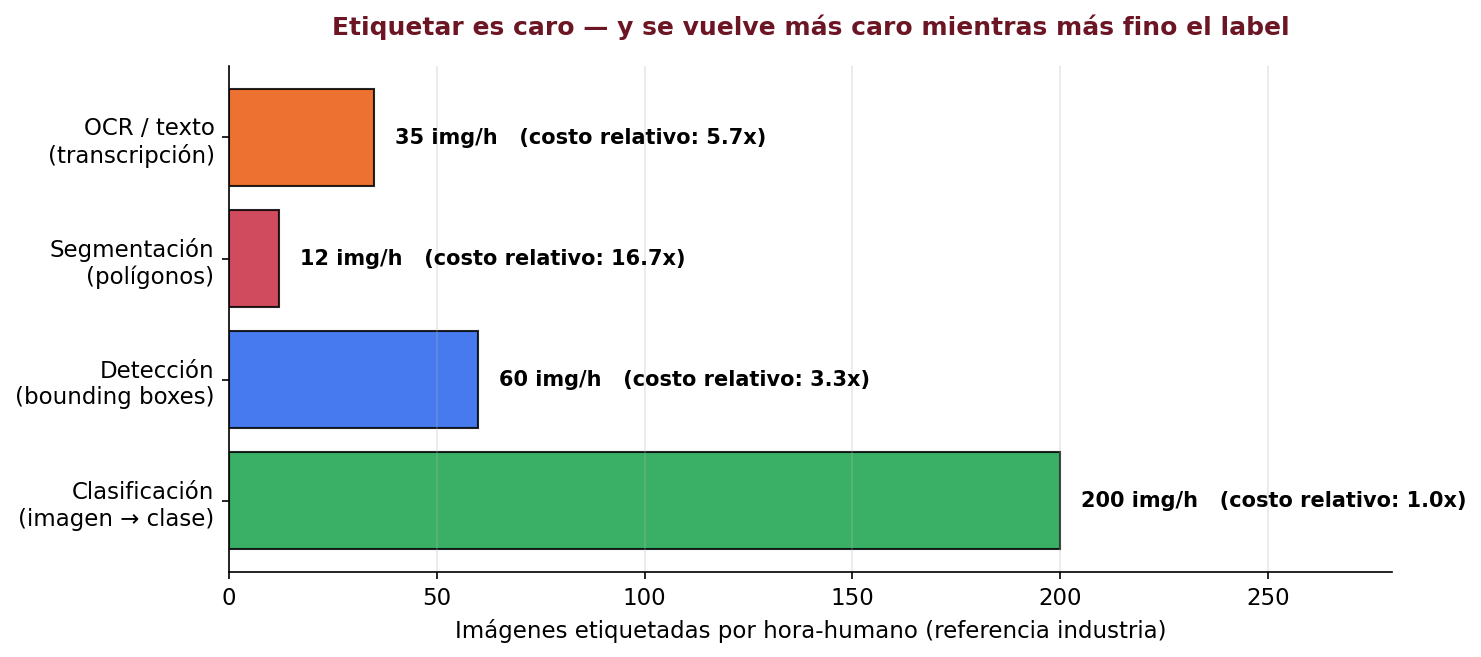
\includegraphics[width=0.92\textwidth]{fig_motivacion_labels.png}
  \end{center}
  \vspace{6pt}
  {\footnotesize
  Una planta de Arca puede generar \textbf{decenas de miles de imágenes al día}. Etiquetar todas para segmentación llevaría \textbf{años de trabajo humano}. La pregunta interesante no es ``cómo etiqueto más rápido'' sino \textbf{``qué puedo aprender de los datos baratos''}.}
\end{frame}

\begin{frame}[shrink]{Esto No Es Nuevo en el Curso}
  \vspace{6pt}
  \begin{center}
    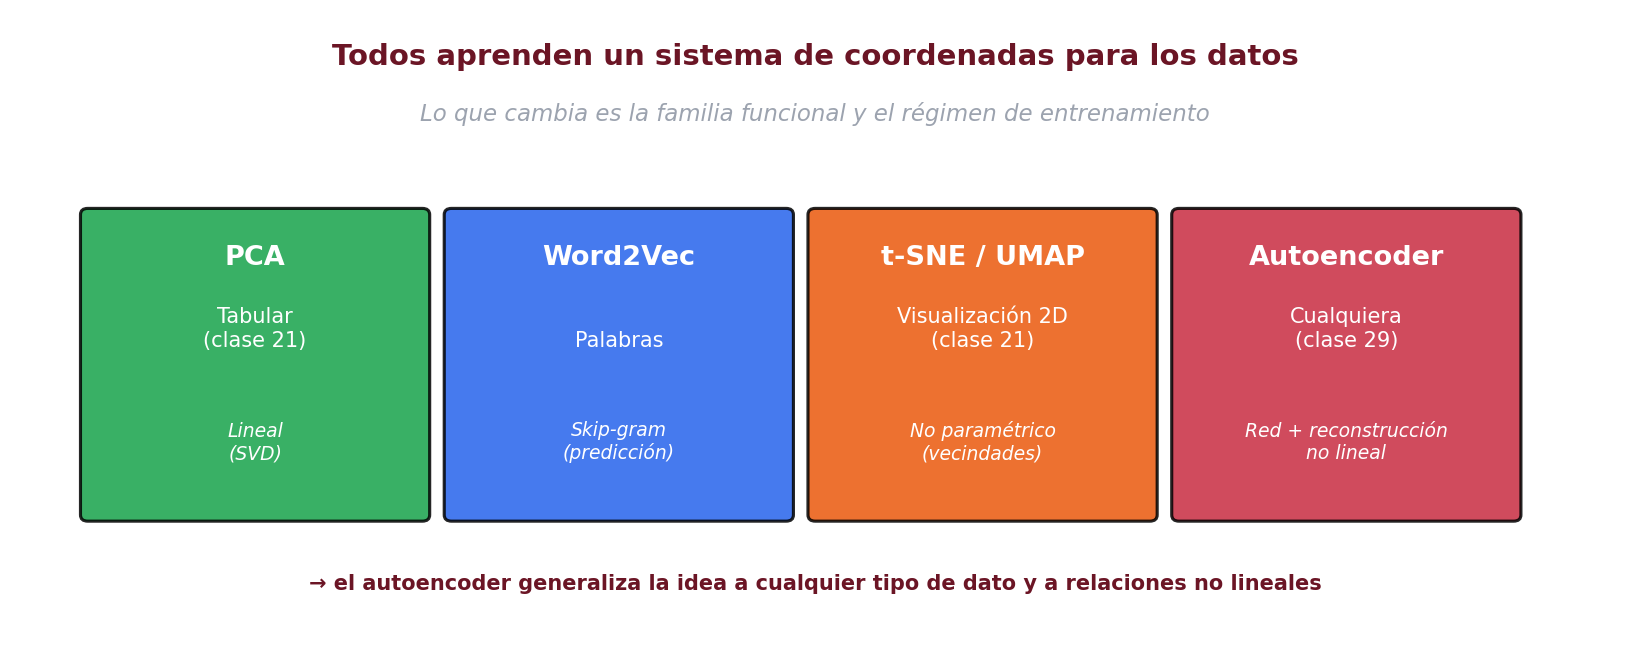
\includegraphics[width=0.95\textwidth]{fig_familia.png}
  \end{center}
  \vspace{4pt}
  {\footnotesize\color{arcaDark}\bfseries
  En clase 19--21 ya vieron K-Means y PCA. El autoencoder es la generalización neuronal y no lineal de la misma idea: aprender un sistema de coordenadas que comprime los datos preservando lo informativo.}
\end{frame}

% ═════════════════════════════════════════════════════════════════════════════
% PARTE 3: QUÉ ES UN AUTOENCODER
% ═════════════════════════════════════════════════════════════════════════════
\sectionframe{Parte 3}{¿Qué Es un Autoencoder?}

\begin{frame}[shrink]{El Nombre Lo Dice Todo}
  \vspace{8pt}
  \begin{center}
  \begin{tikzpicture}
    \node[font=\Huge\bfseries\color{arcaRed}] at (0, 1) {AUTO};
    \node[font=\Huge\bfseries\color{textDark}] at (2.0, 1) {+};
    \node[font=\Huge\bfseries\color{arcaDark}] at (4.5, 1) {ENCODER};

    \node[font=\small\itshape\color{textMuted}, text width=3cm, align=center] at (0, -0.2)
      {por sí mismo,\\sin supervisión};
    \node[font=\small\itshape\color{textMuted}, text width=3cm, align=center] at (4.5, -0.2)
      {codifica datos\\en nuevas\\coordenadas};

    \draw[->, very thick, arcaRed] (-1, -1.8) -- (5.5, -1.8);
    \node[font=\Large\bfseries\color{arcaDark}] at (2.2, -2.3)
      {codificación automática};
  \end{tikzpicture}
  \end{center}
  \vspace{10pt}
  {\small\color{arcaDark}\bfseries
  Es una red que aprende, por sí misma, \emph{cómo codificar} los datos en un sistema de coordenadas distinto al original. No le decimos qué ejes usar --- ella los construye.}
  \vspace{6pt}
  {\footnotesize A ese sistema de coordenadas internas le llamamos \textbf{espacio latente}. El autoencoder es, esencialmente, una máquina para aprender espacios latentes.}
\end{frame}

\begin{frame}[shrink]{El Espacio Latente --- la Pieza Clave}
  \vspace{6pt}
  \begin{center}
    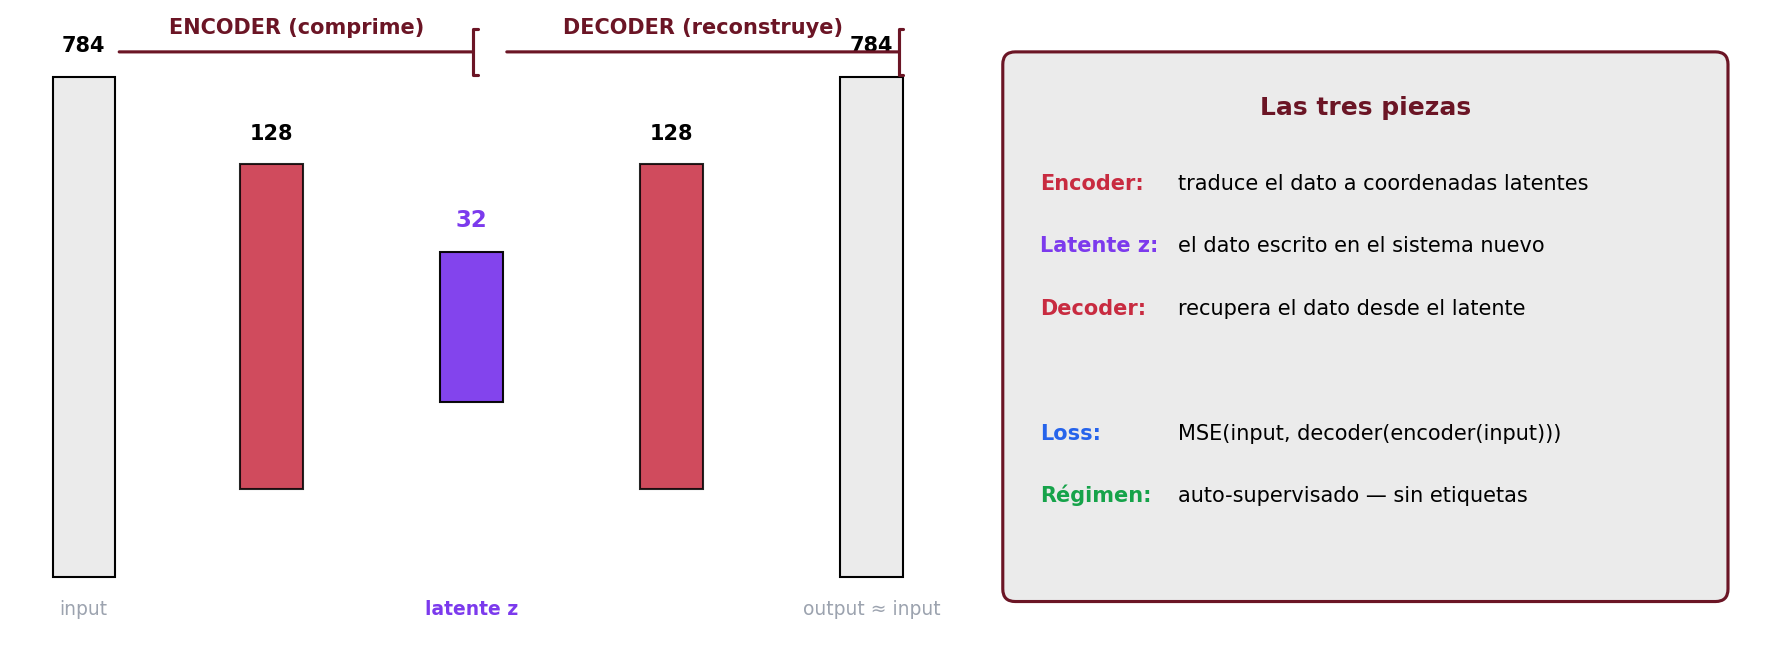
\includegraphics[width=0.95\textwidth]{fig_arquitectura.png}
  \end{center}
  \vspace{4pt}
  {\footnotesize\color{arcaDark}\bfseries
  Tres piezas. Un examen (la reconstrucción) que verifica que el latente captura la información. Un producto (el encoder entrenado) que es lo que usamos después.}
\end{frame}

\begin{frame}[shrink]{La Reconstrucción Es el Examen, No el Producto}
  \vspace{6pt}
  \begin{center}
    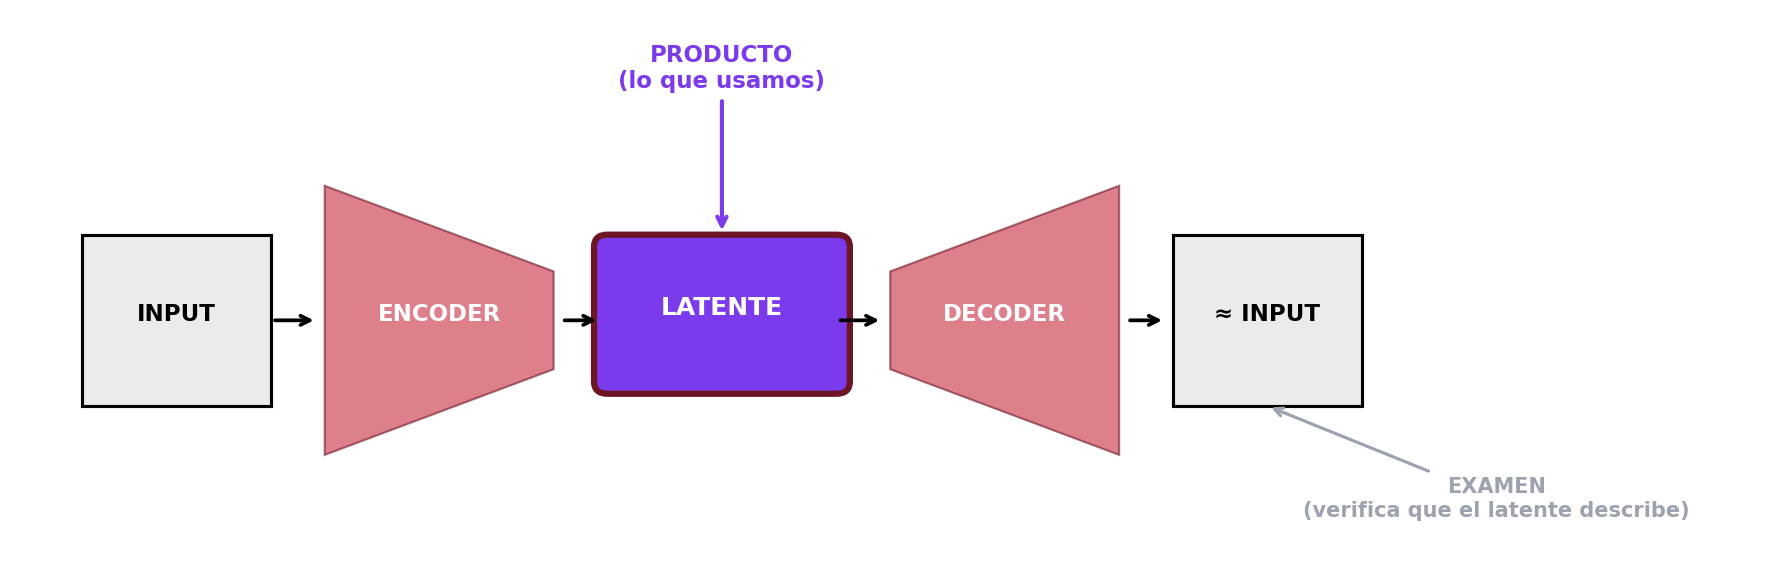
\includegraphics[width=0.92\textwidth]{fig_examen.png}
  \end{center}
  \vspace{4pt}
  \begin{itemize}\setlength\itemsep{2pt}
    \item \textbf{La salida borrosa del decoder NO es lo que nos llevamos.} Es solo la prueba de que el latente puede regenerar el dato.
    \item Lo que se va a producción es \textbf{el encoder entrenado} --- el traductor al espacio latente.
    \item Las aplicaciones (anomalía, denoising, compresión, generación) son distintos \emph{usos} del mismo encoder.
  \end{itemize}
\end{frame}

\begin{frame}[shrink]{Régimen de Entrenamiento: Auto-Supervisado}
  \vspace{8pt}
  \begin{center}
  $\text{Loss}(\theta) \;=\; \text{MSE}\bigl(\,X,\; \text{decoder}_\theta(\text{encoder}_\theta(X))\,\bigr)$
  \end{center}
  \vspace{12pt}
  \begin{itemize}\setlength\itemsep{4pt}
    \item Como el ``label'' es el mismo input, \textbf{no hace falta etiquetar nada}.
    \item Régimen llamado \textbf{auto-supervisado}: la supervisión la generan los datos.
    \item Los modelos modernos tipo BERT, GPT, CLIP, DINOv2 son todos auto-supervisados a su manera. El AE es el caso más claro y didáctico.
    \item Para imágenes en escala $[0, 1]$: capa final \texttt{sigmoid} + loss MSE (o binary crossentropy). Para datos tabulares con valores negativos: capa final \texttt{linear} + MSE.
  \end{itemize}
\end{frame}

\begin{frame}[shrink]{Por Qué Tiene Que Haber Compresión}
  \vspace{8pt}
  \begin{itemize}\setlength\itemsep{6pt}
    \item Si el latente tuviera 784 dimensiones, el encoder podría aprender \textbf{la identidad}: copiar pixel a pixel sin haber descrito nada nuevo.
    \item La compresión a un espacio más pequeño (32, 64, etc.) \textbf{es la restricción} que obliga al encoder a elegir qué información retener.
    \item Lo que sobrevive al cuello es, por construcción, \textbf{lo que distingue una observación de otra} en tus datos.
  \end{itemize}
  \vspace{10pt}
  \begin{center}
  {\color{arcaDark}\bfseries\Large
  ¿Qué es informativo en mis datos?\\[4pt]
  \normalsize\color{textMuted}\itshape El espacio latente entrenado es la respuesta operativa del modelo a esa pregunta.}
  \end{center}
\end{frame}

\begin{frame}[shrink]{Comparación Conceptual con Métodos Previos}
  \vspace{6pt}
  {\footnotesize
  \begin{tabular}{@{}p{2.6cm} p{3.0cm} p{3.0cm} p{4.0cm}@{}}
    \toprule
    \rowcolor{arcaLightGray}
     & \textbf{PCA} & \textbf{Autoencoder lineal} & \textbf{Autoencoder no lineal} \\
    \midrule
    Familia funcional & Lineal & Lineal & Cualquiera (con activaciones) \\
    Entrenamiento & SVD (un paso) & Gradient descent & Gradient descent \\
    Equivalencia & --- & \textbf{$\equiv$ PCA} (mismo óptimo) & Estrictamente más expresivo \\
    Interpretabilidad & Alta (varianza) & Alta & Baja (caja negra) \\
    Ortogonalidad ejes & Garantizada & Garantizada & No \\
    Coste & Barato & Caro & Caro \\
    Captura no linealidad & No & No & \textbf{Sí} \\
    \bottomrule
  \end{tabular}}
  \vspace{14pt}
  {\footnotesize\color{arcaDark}\bfseries
  Regla práctica: PCA primero como baseline. Si la reconstrucción es buena, no hay razón para subir a AE.}
\end{frame}

\begin{frame}[shrink]{Las 5 Estructuras Típicas de un Autoencoder}
  \vspace{6pt}
  {\footnotesize
  \begin{tabular}{@{}p{2.8cm} p{3.1cm} p{3.4cm} p{4.0cm}@{}}
    \toprule
    \rowcolor{arcaLightGray}
    \textbf{Layout} & \textbf{Encoder} & \textbf{Decoder} & \textbf{Cuándo usarlo} \\
    \midrule
    Dense AE & \texttt{Dense} & \texttt{Dense} & Tabular, vectores, embeddings \\
    Conv AE & \texttt{Conv2D + Pool} & \texttt{Conv2D + UpSampling} & Imágenes (hoy con MNIST) \\
    Conv AE híbrido & \texttt{Conv2D + Pool $\to$ Flatten $\to$ Dense} & \texttt{Dense $\to$ Reshape $\to$ Conv} & Imágenes con latente vectorial chico \\
    U-Net & \texttt{Conv2D + Pool} & \texttt{Conv + Up + skip} & Segmentación pixel-wise \\
    Seq2Seq AE & \texttt{LSTM / Transformer} & \texttt{LSTM / Transformer} & Series, texto, audio (Módulo 5) \\
    \bottomrule
  \end{tabular}}
  \vspace{8pt}
  \begin{itemize}\setlength\itemsep{2pt}
    \item Todos comparten: input shape libre, encoder reductor, bottleneck, decoder \emph{aproximadamente} simétrico, output igual al input shape.
    \item El decoder NO tiene que ser espejo exacto del encoder. Decisión común: decoder más simple (menos parámetros, entrena más rápido).
    \item Capa final con activación distinta al resto: \texttt{sigmoid} si los datos están en $[0,1]$, \texttt{linear} si pueden ser negativos.
  \end{itemize}
\end{frame}

\begin{frame}[fragile,shrink]{Las 6 Capas Keras de Todo Autoencoder de Imágenes}
  \vspace{4pt}
  {\footnotesize
  \begin{tabular}{@{}p{4.0cm} p{6.0cm} p{3.5cm}@{}}
    \toprule
    \rowcolor{arcaLightGray}
    \textbf{Capa} & \textbf{Qué hace} & \textbf{Dónde aparece} \\
    \midrule
    \texttt{Input(shape=...)}    & Declara el shape (sin batch dim) & Primera línea siempre \\
    \texttt{Dense(n, activation)} & Fully-connected con $n$ unidades & Dense AE, bottlenecks \\
    \texttt{Conv2D(n, k, padding)} & $n$ filtros de $k\times k$ & Encoder Conv AE \\
    \texttt{MaxPooling2D(2)}      & Reduce dimensión espacial a la mitad & Encoder Conv AE \\
    \texttt{UpSampling2D(2)}      & Duplica dimensión espacial & Decoder Conv AE \\
    \texttt{Conv2DTranspose(n, k, strides)} & ``Conv inversa'' aprendida & Decoder alternativo \\
    \bottomrule
  \end{tabular}}
  \vspace{8pt}
  \begin{pyblock}
# Sequential -- para 95% de los AE
model = Sequential([
    layers.Input(shape=(28, 28, 1)),
    layers.Conv2D(16, 3, activation="relu", padding="same"),
    layers.MaxPooling2D(2),
    # ...
])
# Functional -- solo cuando necesites separar encoder/decoder o skip connections
  \end{pyblock}
\end{frame}

% ═════════════════════════════════════════════════════════════════════════════
% PARTE 4: AE EN MNIST
% ═════════════════════════════════════════════════════════════════════════════
\sectionframe{Parte 4}{Primer Autoencoder en MNIST}

\begin{frame}[fragile,shrink]{Dense AE con \texttt{Sequential} --- lo Más Simple}
  \vspace{-4pt}
  \begin{pyblock}
from tensorflow.keras import Sequential, layers

LATENT_DIM = 32

ae = Sequential([
    layers.Input(shape=(784,)),
    # Encoder
    layers.Dense(128, activation="relu"),
    layers.Dense(LATENT_DIM, activation="relu"),   # bottleneck
    # Decoder (simetrico)
    layers.Dense(128, activation="relu"),
    layers.Dense(784, activation="sigmoid"),
], name="dense_autoencoder")

ae.compile(optimizer="adam", loss="mse")
  \end{pyblock}
  \vspace{4pt}
  {\footnotesize 5 capas, $\sim$225K parámetros, sigmoid final para mantener salida en $[0, 1]$.}
\end{frame}

\begin{frame}[fragile,shrink]{Entrenamiento: \texttt{fit(X, X)} --- la Firma del AE}
  \vspace{-4pt}
  \begin{pyblock}
# El target es el mismo X. No hay y_train.
ae.fit(X_train_flat, X_train_flat,
        epochs=10, batch_size=256, validation_split=0.1)
  \end{pyblock}
  \vspace{8pt}
  \begin{itemize}\setlength\itemsep{4pt}
    \item \texttt{fit(X, X)} en lugar de \texttt{fit(X, y)} es \textbf{el indicador visible} de que estás entrenando sin etiquetas.
    \item La loss MSE compara pixel a pixel input contra output.
    \item Sin GPU: $\sim$30 segundos. Con T4: 5 segundos.
  \end{itemize}
\end{frame}

\begin{frame}[shrink]{Resultado --- Reconstrucciones Borrosas Pero Identificables}
  \vspace{6pt}
  \begin{itemize}\setlength\itemsep{4pt}
    \item Compresión 24$\times$ (de 784 a 32 dimensiones). La forma sobrevive; el grano fino se pierde.
    \item La borrosidad viene del MSE: el mínimo del error promedio entre todos los 3 plausibles es un 3 \emph{suavizado}.
    \item La memoria del encoder no es por píxel sino \textbf{por estructura} --- bordes, simetrías, regiones cerradas.
    \item En el notebook: \texttt{ae.predict(x)} sobre 10 imágenes random. La reconstrucción conserva identidad de clase, pierde detalle fino.
  \end{itemize}
\end{frame}

\begin{frame}[shrink]{Compresión por Dígito --- No Todas las Clases Comprimen Igual}
  \vspace{2pt}
  \begin{center}
    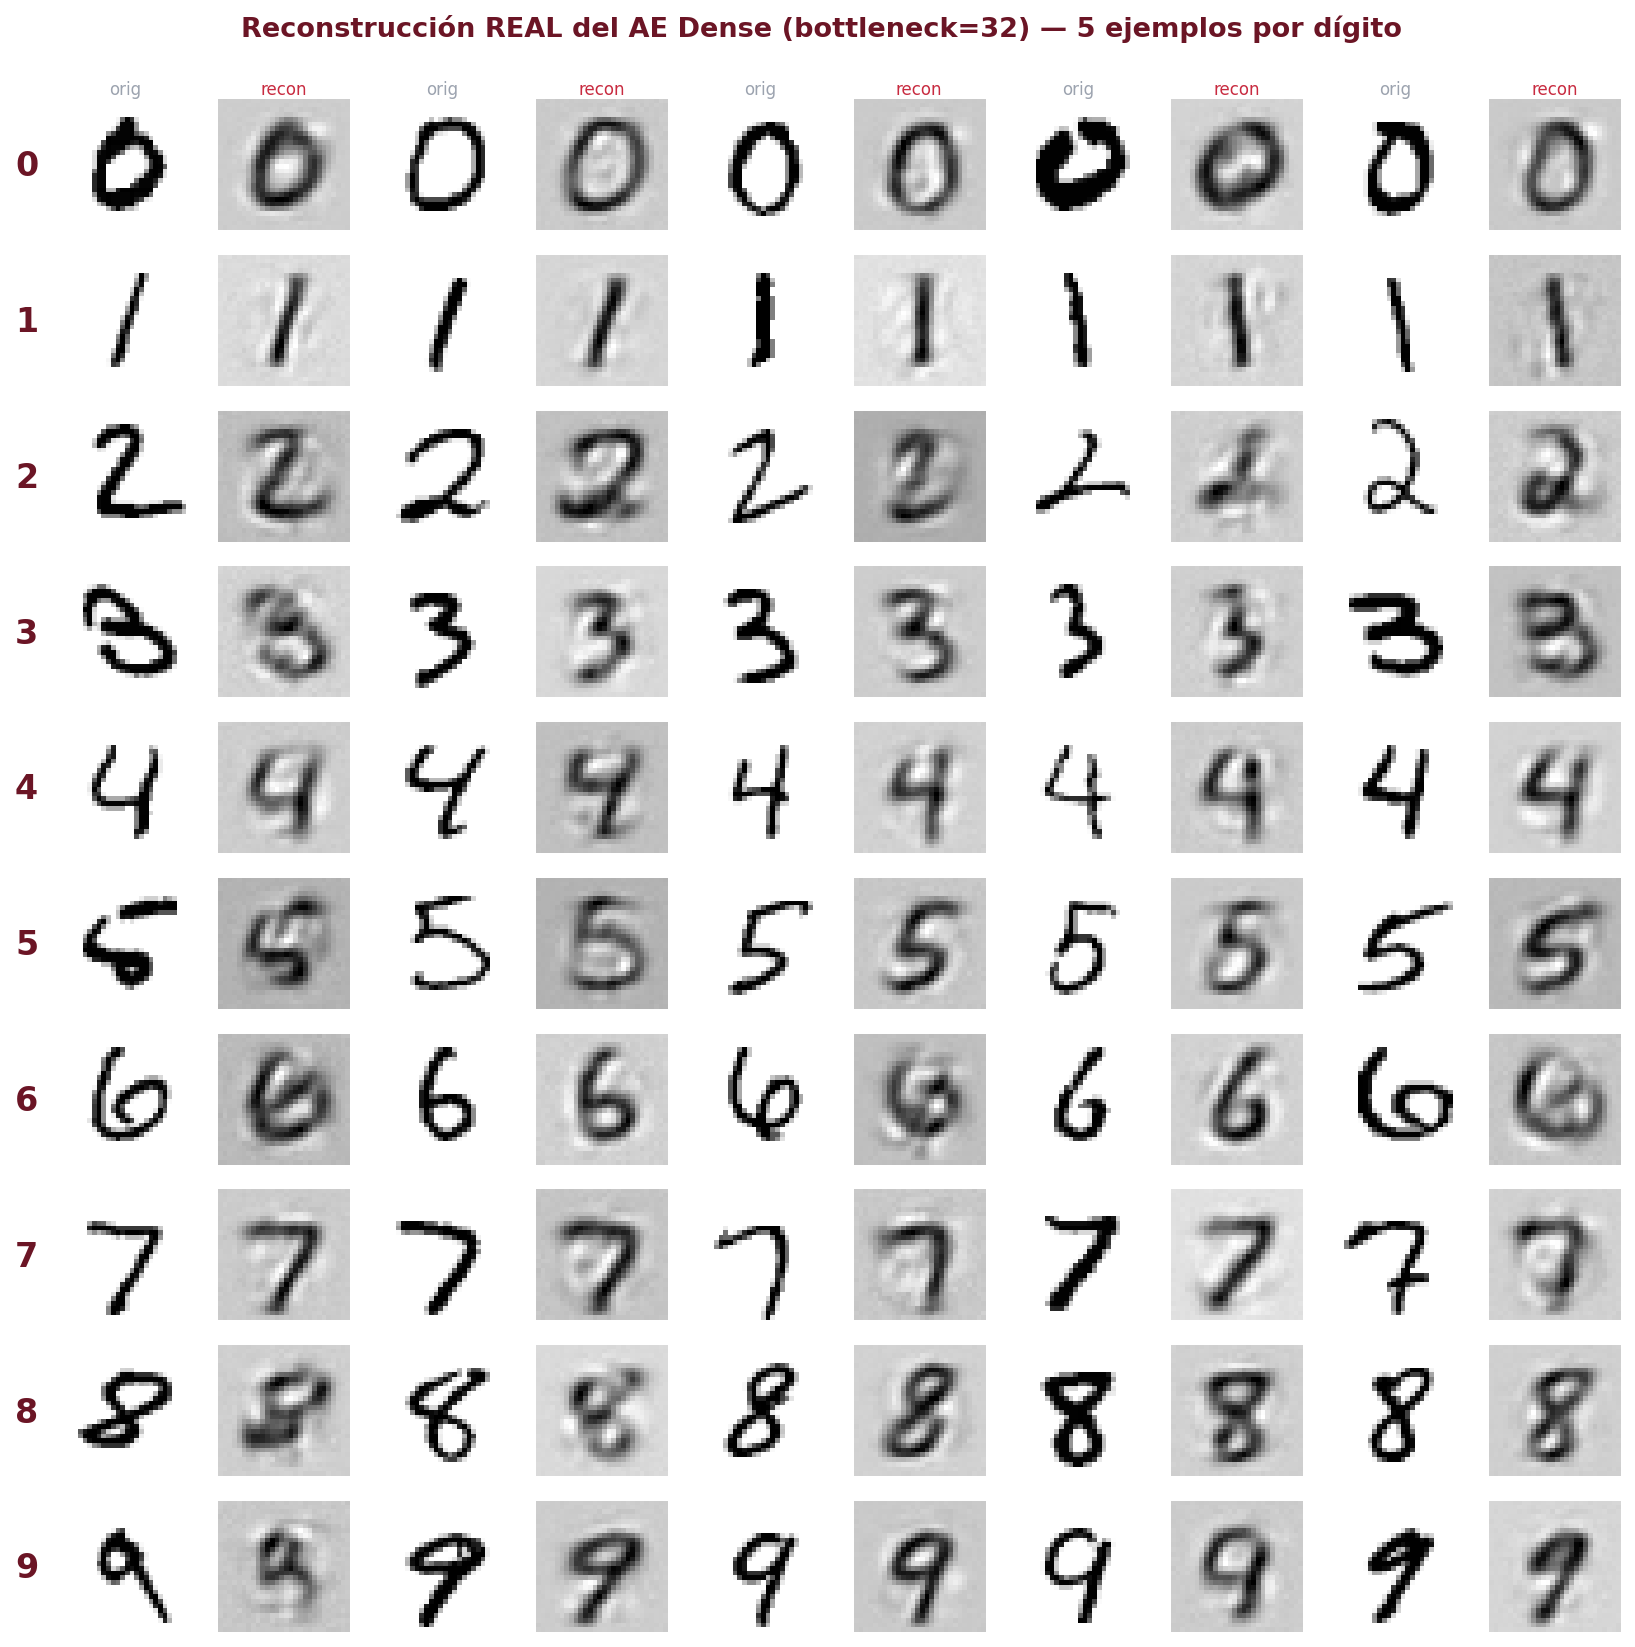
\includegraphics[width=0.52\textwidth]{fig_compresion_por_digito.png}
  \end{center}
  \vspace{-2pt}
  {\footnotesize\color{arcaDark}\bfseries
  Dígitos ``fáciles'' (1, 0, 7) reconstruyen casi exacto. Dígitos ``difíciles'' (5, 8) salen visiblemente borrosos. Esa heterogeneidad NO es ruido --- es información estructural sobre la geometría del manifold.}
\end{frame}

\begin{frame}[shrink]{Qué Aprende el Latente --- Visualización 2D}
  \vspace{4pt}
  \begin{center}
    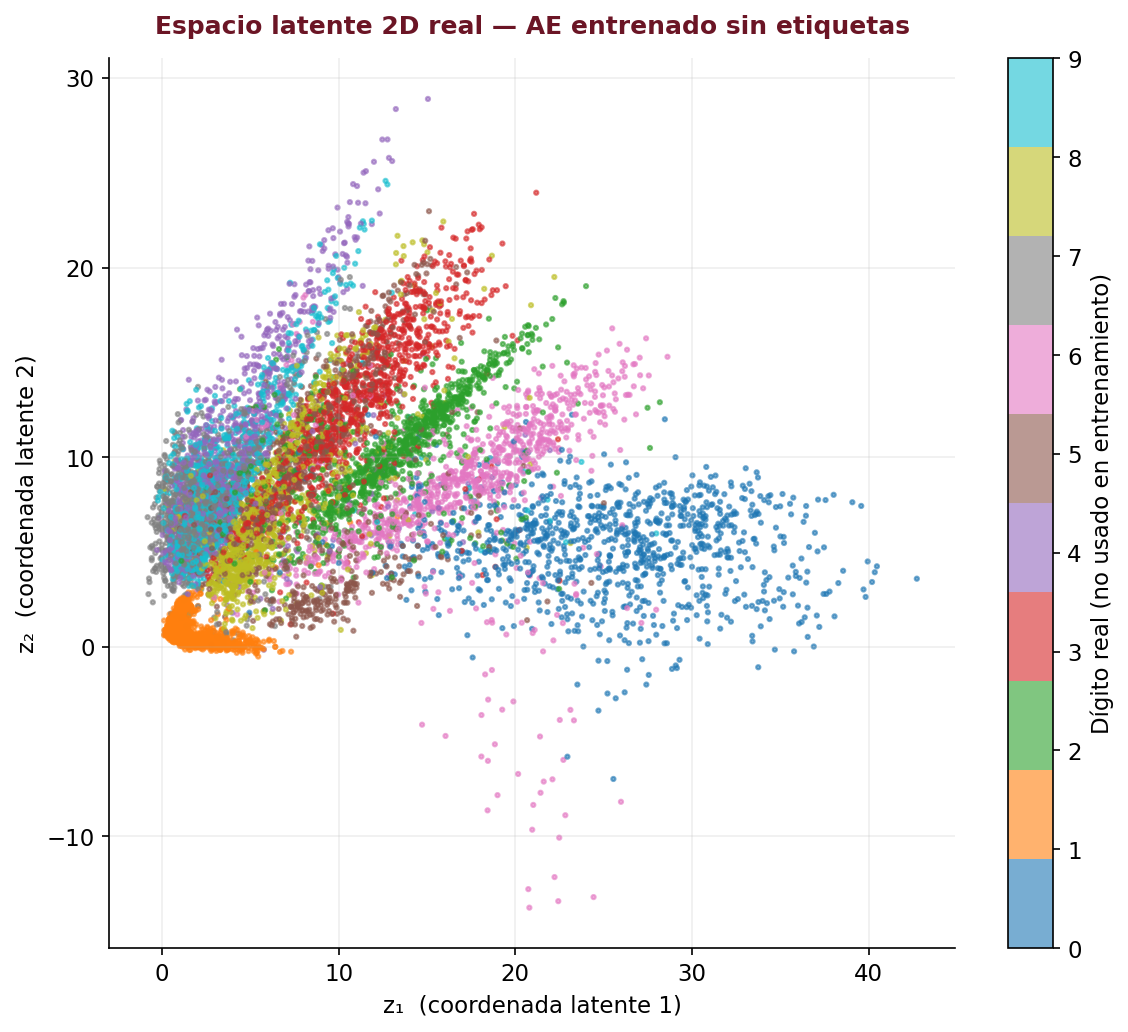
\includegraphics[width=0.62\textwidth]{fig_latente_2d.png}
  \end{center}
  \vspace{2pt}
  {\footnotesize\color{arcaDark}\bfseries
  Sin haber visto las etiquetas, el encoder construye coordenadas donde los dígitos se separan en grupos. La estructura de clases existe en los datos mismos --- el encoder solo la refleja.}
\end{frame}

\begin{frame}[shrink]{PCA vs Autoencoder --- Misma Tarea, Resultado Distinto}
  \vspace{4pt}
  \begin{center}
    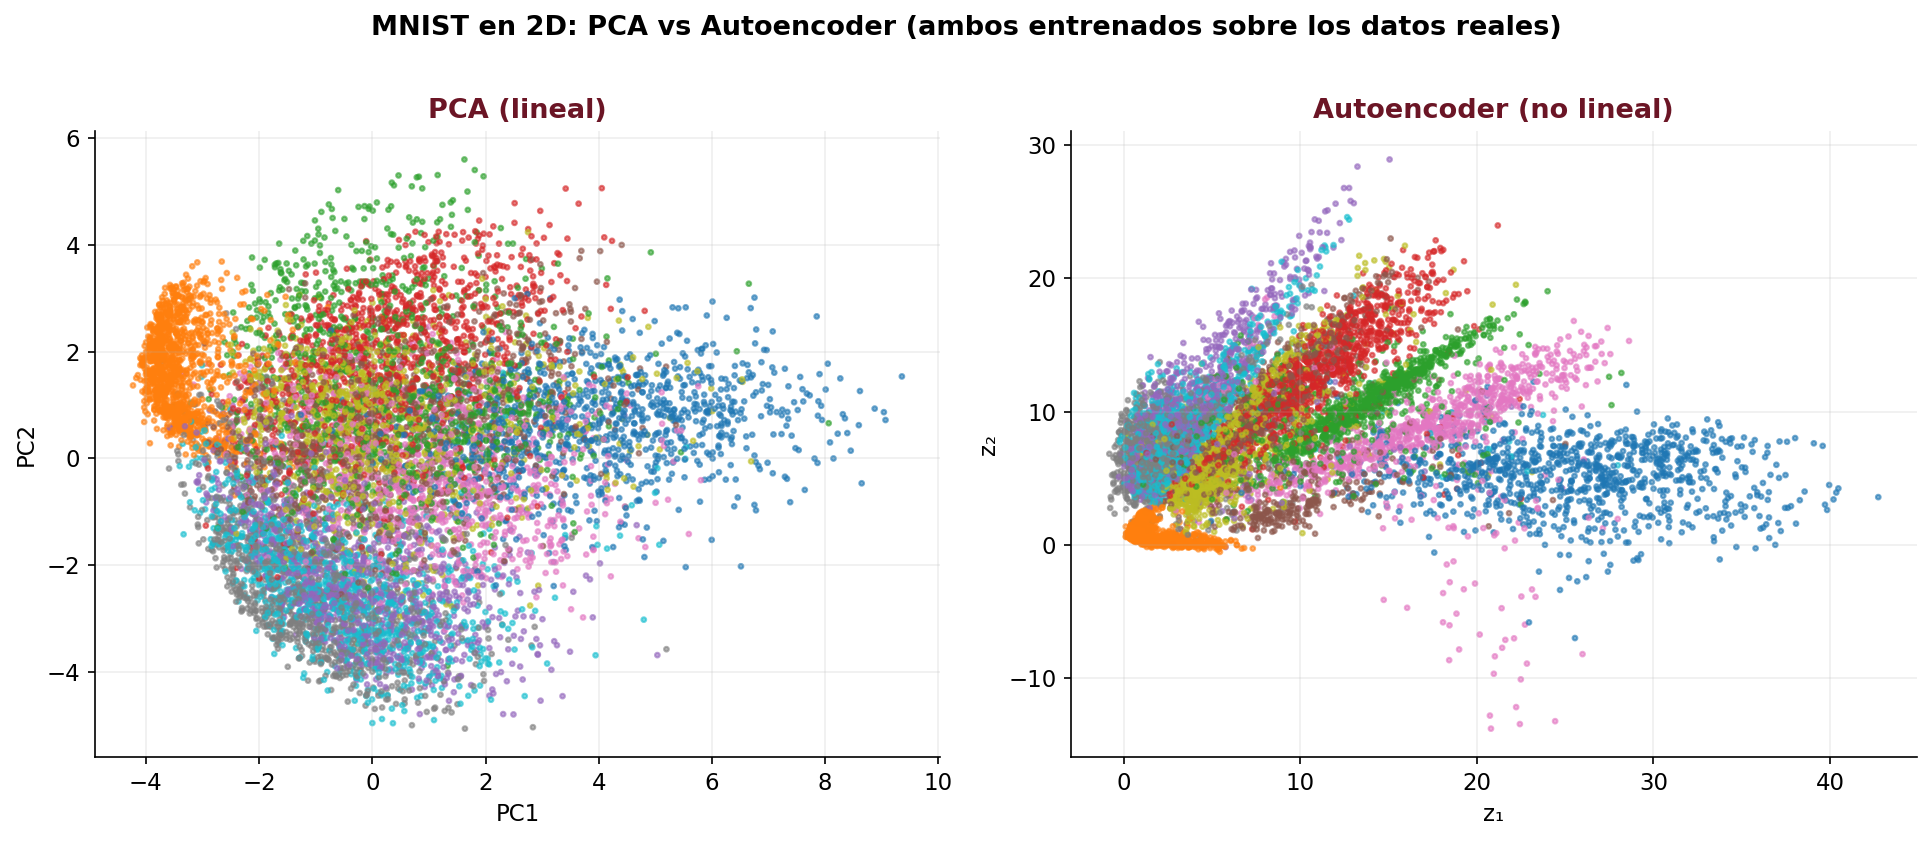
\includegraphics[width=0.95\textwidth]{fig_pca_vs_ae.png}
  \end{center}
  \vspace{2pt}
  \begin{itemize}\setlength\itemsep{2pt}
    \item PCA: ejes lineales de mayor varianza. Cluster mezclados.
    \item AE: ejes pueden curvarse para acomodar la estructura $\to$ clusters más separados.
    \item \textbf{Ventaja operativa del AE sobre t-SNE}: encoder \emph{paramétrico} --- podemos pasarle datos nuevos sin reentrenar.
  \end{itemize}
\end{frame}

\begin{frame}[shrink]{Conv Autoencoder --- Arquitectura}
  \vspace{2pt}
  \begin{center}
    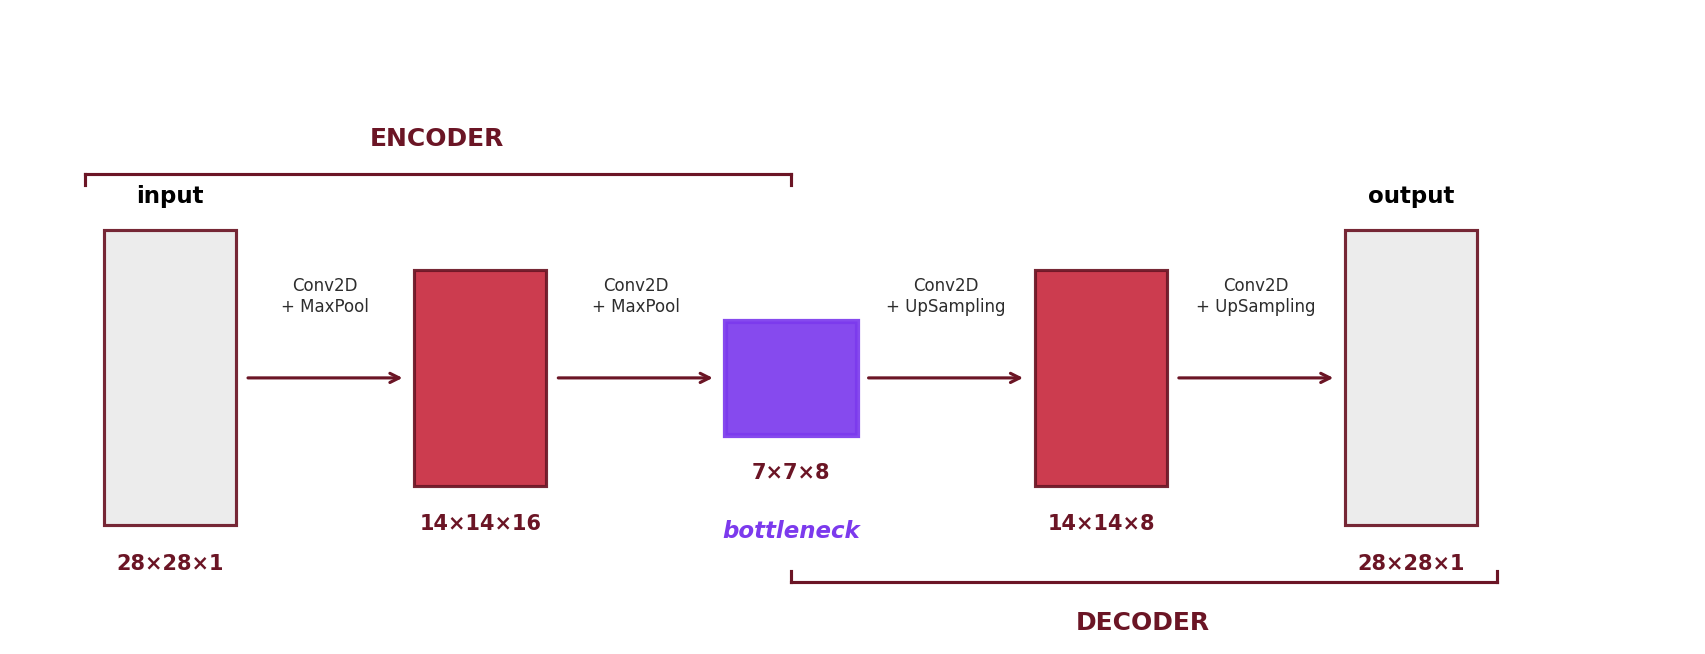
\includegraphics[width=0.92\textwidth]{fig_conv_ae.png}
  \end{center}
  \vspace{2pt}
  \begin{itemize}\setlength\itemsep{2pt}
    \item Encoder: \texttt{Conv2D + MaxPooling2D} reduce la imagen a la mitad cada paso.
    \item Bottleneck: 7$\times$7$\times$8 = 392 valores (vs 784 del input).
    \item Decoder: \texttt{Conv2D + UpSampling2D} agranda al doble cada paso. Alternativa: \texttt{Conv2DTranspose} (aprende cómo agrandar, lo usa U-Net).
  \end{itemize}
\end{frame}

% ═════════════════════════════════════════════════════════════════════════════
% PARTE 5: COMPRESIÓN Y PRETRAINING
% ═════════════════════════════════════════════════════════════════════════════
\sectionframe{Parte 5}{Aplicación 1 --- Compresión y Pretraining}

\begin{frame}[shrink]{El Encoder Entrenado Es el Activo}
  \vspace{6pt}
  \begin{itemize}\setlength\itemsep{4pt}
    \item Después de entrenar el AE, lo que ganamos es \textbf{el encoder} --- un traductor de input a 32 números informativos.
    \item Ese encoder vio millones de muestras sin label y aprendió \textbf{qué es informativo en ese dominio}.
    \item Si después tenemos un problema supervisado con \textbf{pocos labels}, el encoder ya hizo la mitad del trabajo.
  \end{itemize}
  \vspace{10pt}
  \begin{center}
  {\footnotesize
  \begin{tabular}{@{}p{4.2cm} p{4.0cm} p{4.5cm}@{}}
    \toprule
    \rowcolor{arcaLightGray}
     & \textbf{Sin pretraining} & \textbf{Con pretraining} \\
    \midrule
    Input al clasificador & 784 píxeles crudos & 32 features del encoder \\
    Parámetros del clasificador & Muchos (entrada grande) & Pocos (entrada compacta) \\
    Data labeled necesaria & Miles & Cientos pueden bastar \\
    Data sin label aprovechada & 0 & Toda la que tengas \\
    \bottomrule
  \end{tabular}}
  \end{center}
\end{frame}

\begin{frame}[shrink]{Pretraining --- el Flujo Completo}
  \vspace{2pt}
  \begin{center}
    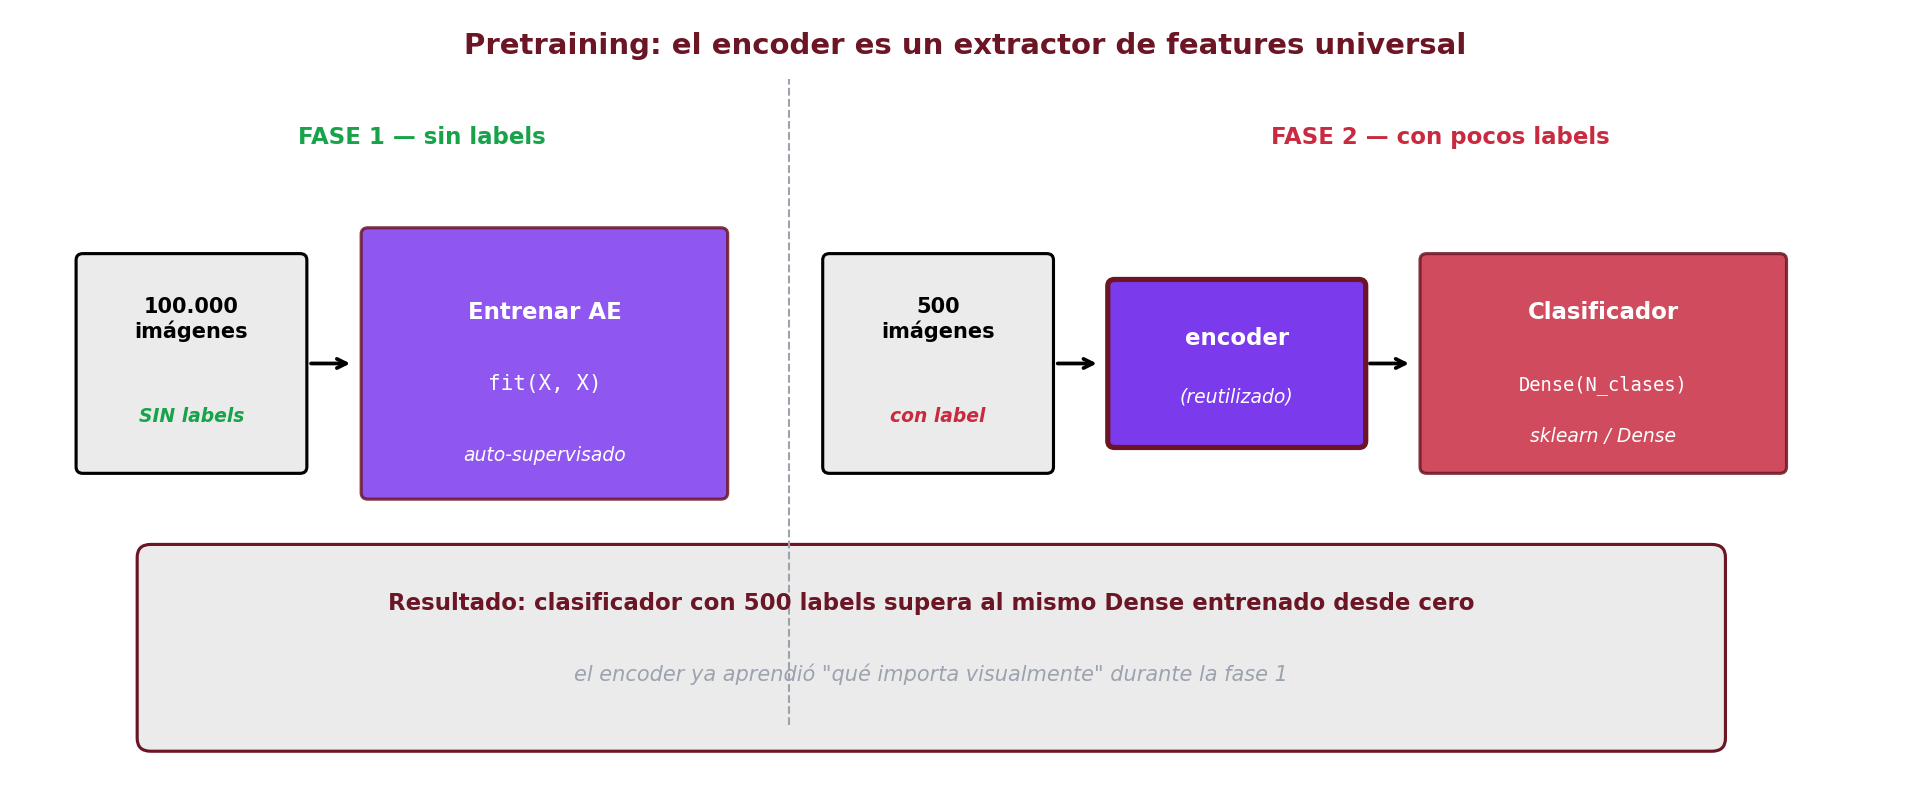
\includegraphics[width=0.96\textwidth]{fig_pretraining.png}
  \end{center}
\end{frame}

\begin{frame}[fragile,shrink]{Demo en MNIST --- 200 Labels vs 60.000 Sin Label}
  \vspace{-4pt}
  \begin{pyblock}
# Pretraining: el AE ya esta entrenado en 60.000 imagenes SIN labels
features_lab  = encoder.predict(X_lab)        # 200 imagenes -> (200, 32)
features_test = encoder.predict(X_test_flat)

# Clasificador pequeno sobre features comprimidas
clf = Sequential([
    layers.Input(shape=(32,)),
    layers.Dense(32, activation="relu"),
    layers.Dense(10, activation="softmax"),
])
clf.compile(optimizer="adam", loss="sparse_categorical_crossentropy",
             metrics=["accuracy"])
clf.fit(features_lab, y_lab, epochs=30, batch_size=32)

# Resultado esperado: +3 a +8 puntos de accuracy vs entrenar el mismo
# clasificador directamente sobre los 784 pixels crudos.
  \end{pyblock}
\end{frame}

\begin{frame}[shrink]{Otros Usos del Encoder Entrenado en Producción}
  \vspace{4pt}
  {\footnotesize
  \begin{tabular}{@{}p{4.0cm} p{9.5cm}@{}}
    \toprule
    \rowcolor{arcaLightGray}
    \textbf{Caso de uso} & \textbf{Cómo se usa el encoder} \\
    \midrule
    Buscar productos similares a partir de una foto
      & Una tienda con 10 millones de productos. En lugar de comparar cada foto píxel por píxel, comprimes cada una a 64 números. La búsqueda \emph{``encuéntrame productos parecidos a esta foto''} se vuelve comparar vectores de 64 contra 64. \\
    Sistemas de recomendación (Netflix, e-commerce)
      & Entrenas el AE sobre la matriz ``qué usuario vio qué película''. El encoder aprende las dimensiones de gusto de cada usuario. Recomendar = encontrar películas cuyo vector esté cerca del vector del usuario. \\
    Compresión de imágenes y video
      & JPEG clásico usa una transformación matemática fija (DCT). Versiones nuevas usan un AE: encoder reduce la imagen a pocos números que se transmiten; el receptor pasa esos números por el decoder. \\
    Reducir vectores grandes para almacenarlos
      & Modelos de lenguaje grandes producen vectores de 768 números por texto. Con cientos de millones de textos, almacenar tanto es caro. Un AE los comprime a 64 manteniendo qué tan parecidos son entre sí. \\
    Aprovechar datos sin etiquetar
      & El caso que vimos en la slide anterior. Entrenas el AE con todos los datos que tengas (sin etiquetar). Después usas su encoder para alimentar un clasificador chico con las pocas etiquetas disponibles. \\
    \bottomrule
  \end{tabular}}
  \vspace{8pt}
  {\footnotesize\color{arcaDark}\bfseries
  Regla práctica: si tienes muchos datos sin etiqueta y pocas etiquetas, o si vas a resolver el mismo problema varias veces, entrenar primero un AE y reutilizar su encoder casi siempre ayuda.}
\end{frame}

% ═════════════════════════════════════════════════════════════════════════════
% PARTE 6: DENOISING
% ═════════════════════════════════════════════════════════════════════════════
\sectionframe{Parte 6}{Aplicación 2 --- Denoising}

\begin{frame}[shrink]{Variación del Entrenamiento, No de la Arquitectura}
  \vspace{4pt}
  \begin{center}
    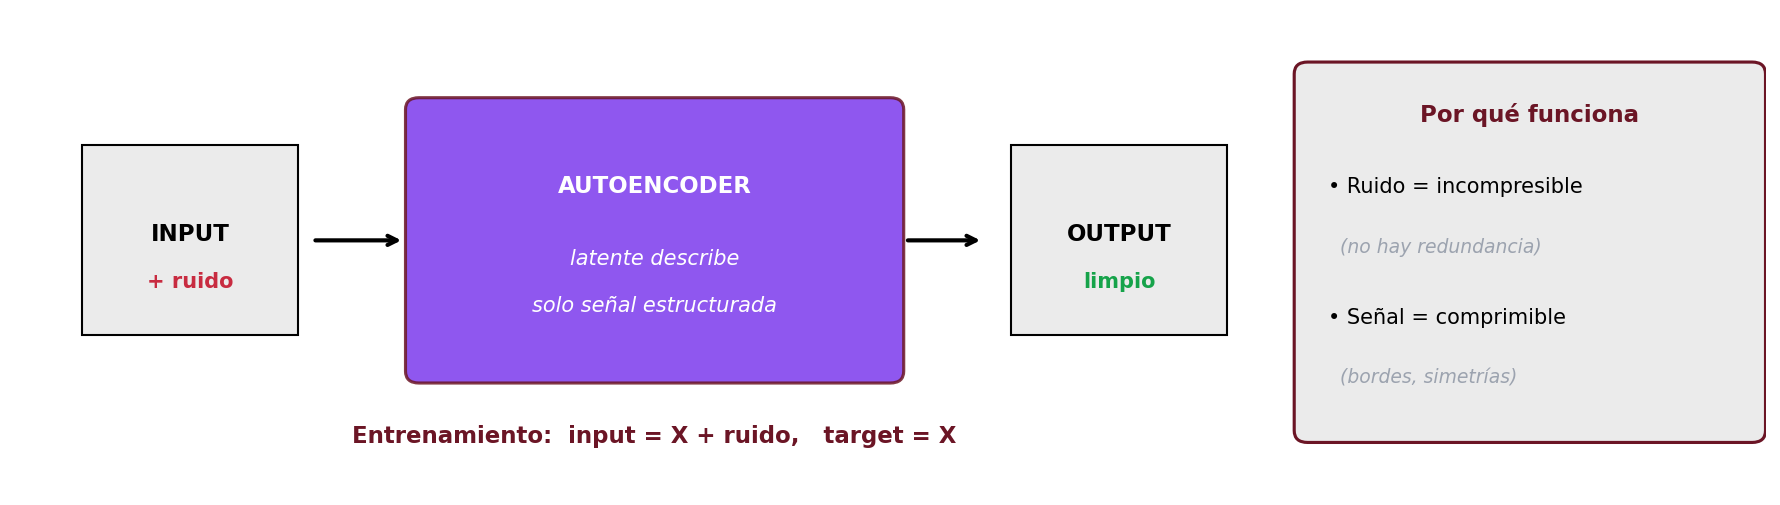
\includegraphics[width=0.95\textwidth]{fig_denoising.png}
  \end{center}
  \vspace{6pt}
  \begin{itemize}
    \item Arquitectura: \textbf{idéntica} al Conv AE de antes.
    \item Lo único que cambia: el input al \texttt{fit} es la versión degradada; el target sigue siendo la versión limpia.
  \end{itemize}
\end{frame}

\begin{frame}[fragile,shrink]{Código: Una Sola Línea de Diferencia}
  \vspace{-4pt}
  \begin{pyblock}
# Generar versiones degradadas (ruido gaussiano)
X_train_noisy = np.clip(X_train + 0.4 * np.random.normal(size=X_train.shape),
                        0, 1)

# La unica diferencia: input ruidoso, target limpio
denoising_ae.fit(X_train_noisy, X_train,      # <-- input != target
                  epochs=8, batch_size=256,
                  validation_data=(X_test_noisy, X_test))
  \end{pyblock}
\end{frame}

\begin{frame}[shrink]{Cómo Se Ve Ese Ruido (Visualización)}
  \vspace{4pt}
  \begin{center}
    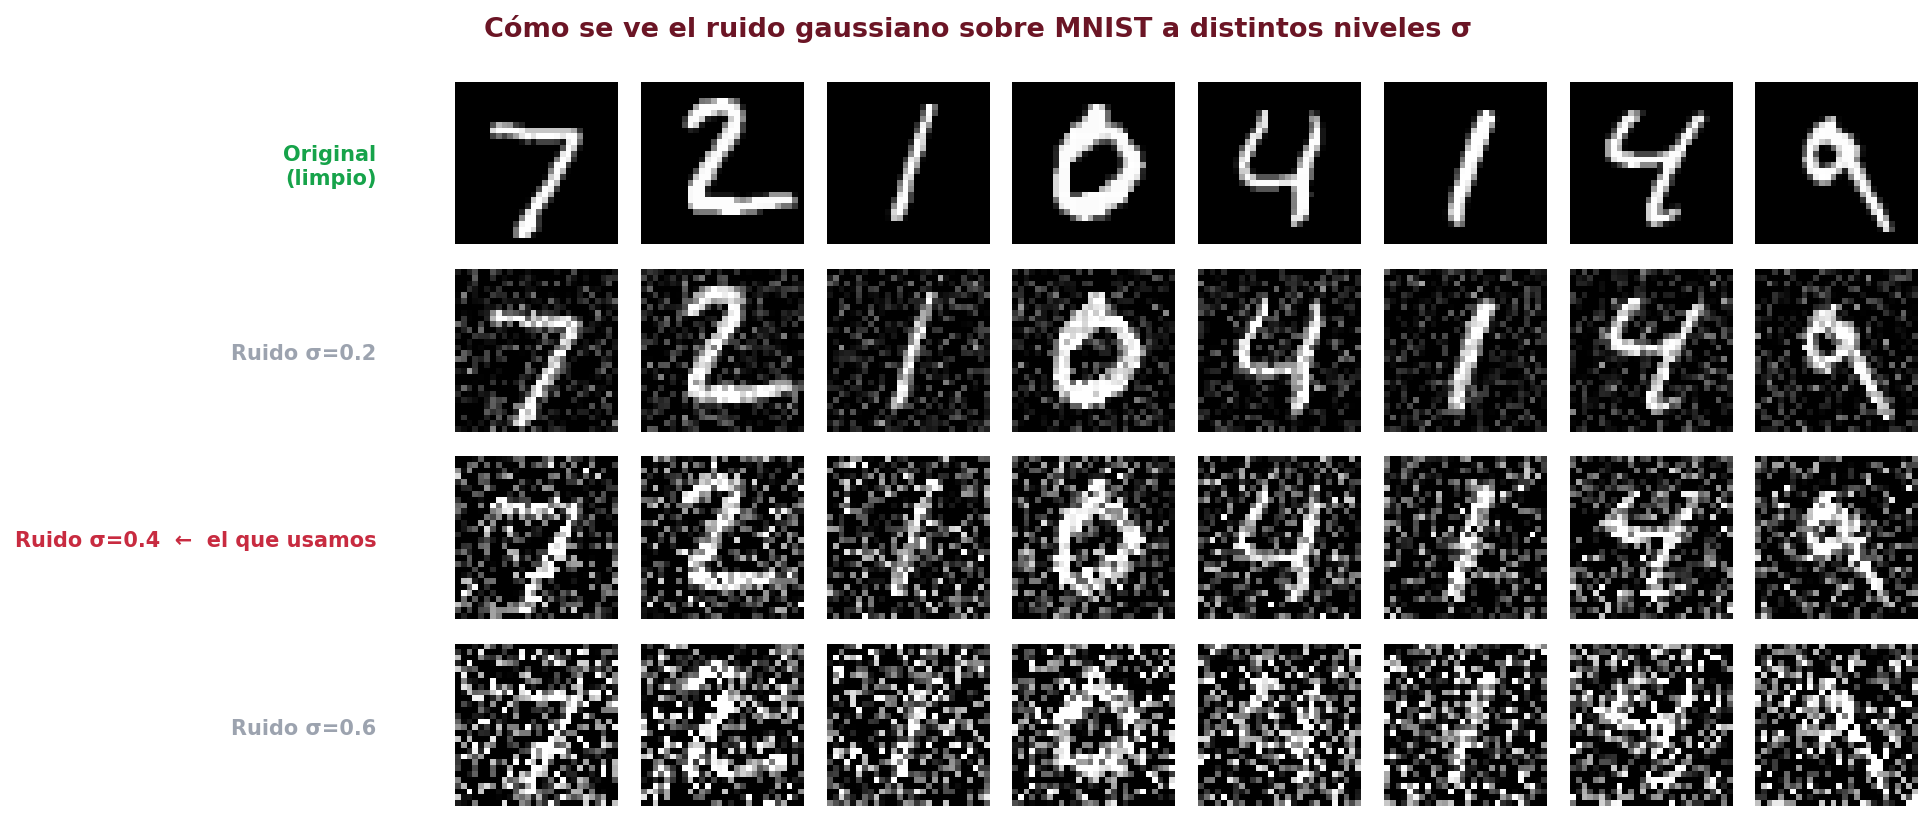
\includegraphics[width=0.92\textwidth]{fig_ruido_ejemplo.png}
  \end{center}
  \vspace{2pt}
  {\footnotesize\color{arcaDark}\bfseries
  El parámetro $\sigma$ controla la intensidad del ruido. Usamos $\sigma = 0.4$ porque deja el dígito todavía reconocible pero ya difícil de leer --- el reto justo para que el AE tenga que aprender a reconstruir la estructura subyacente.}
\end{frame}

\begin{frame}[shrink]{Por Qué el Denoising AE Funciona}
  \vspace{8pt}
  \begin{itemize}\setlength\itemsep{6pt}
    \item El ruido gaussiano es \textbf{estructuralmente incompresible}: cada píxel se sortea independiente, no hay redundancia entre vecinos.
    \item La señal subyacente \textbf{sí} se comprime: el dígito está hecho de trazos coherentes, regiones cerradas, simetrías locales.
    \item El espacio latente del autoencoder tiene 32 dimensiones (mucho menos que los 784 del input). Esas 32 dimensiones se entrenan para describir lo que es comprimible.
    \item El ruido no logra entrar al latente porque no hay coordenadas disponibles para él. El decoder reconstruye desde el latente y devuelve solo la parte estructurada.
  \end{itemize}
\end{frame}

\begin{frame}[shrink]{Aplicaciones Reales --- Datasets y Dominios}
  \vspace{4pt}
  {\footnotesize
  \begin{tabular}{@{}p{3.3cm} p{3.8cm} p{2.8cm} p{3.5cm}@{}}
    \toprule
    \rowcolor{arcaLightGray}
    \textbf{Dataset / Dominio} & \textbf{Tipo de degradación} & \textbf{Métrica} & \textbf{Aplicación industrial} \\
    \midrule
    \textbf{DIBCO} & Manuscritos antiguos, manchas, transparencia & F-Measure & Digitalización de archivos \\
    \textbf{SIDD / DND} & Ruido real de cámaras móviles (Samsung, Sony) & PSNR / SSIM & Procesamiento de fotos \\
    \textbf{VoiceBank-DEMAND} & Voz + ruido de fondo (espectrogramas) & PESQ / STOI & Telefonía, call centers \\
    \textbf{Low-dose CT (Mayo)} & Ruido Poisson de baja dosis & PSNR / SSIM & Imagenología médica \\
    \textbf{CSBDeep / Noise2Noise} & Microscopía de fluorescencia & PSNR & Investigación biológica \\
    \textbf{Sensores industriales} & Ruido eléctrico, vibración & MSE & Mantenimiento predictivo \\
    \bottomrule
  \end{tabular}}
  \vspace{8pt}
  {\footnotesize\color{arcaDark}\bfseries
  Patrón común: en cada caso existe un dataset público con pares (sucio, limpio) o (sucio, otro sucio) que permite entrenar el AE para ese tipo de degradación específico.}
\end{frame}

\begin{frame}[shrink]{Denoising No Es Solo Para Imágenes --- Series Temporales (Conv1D)}
  \vspace{4pt}
  \begin{center}
    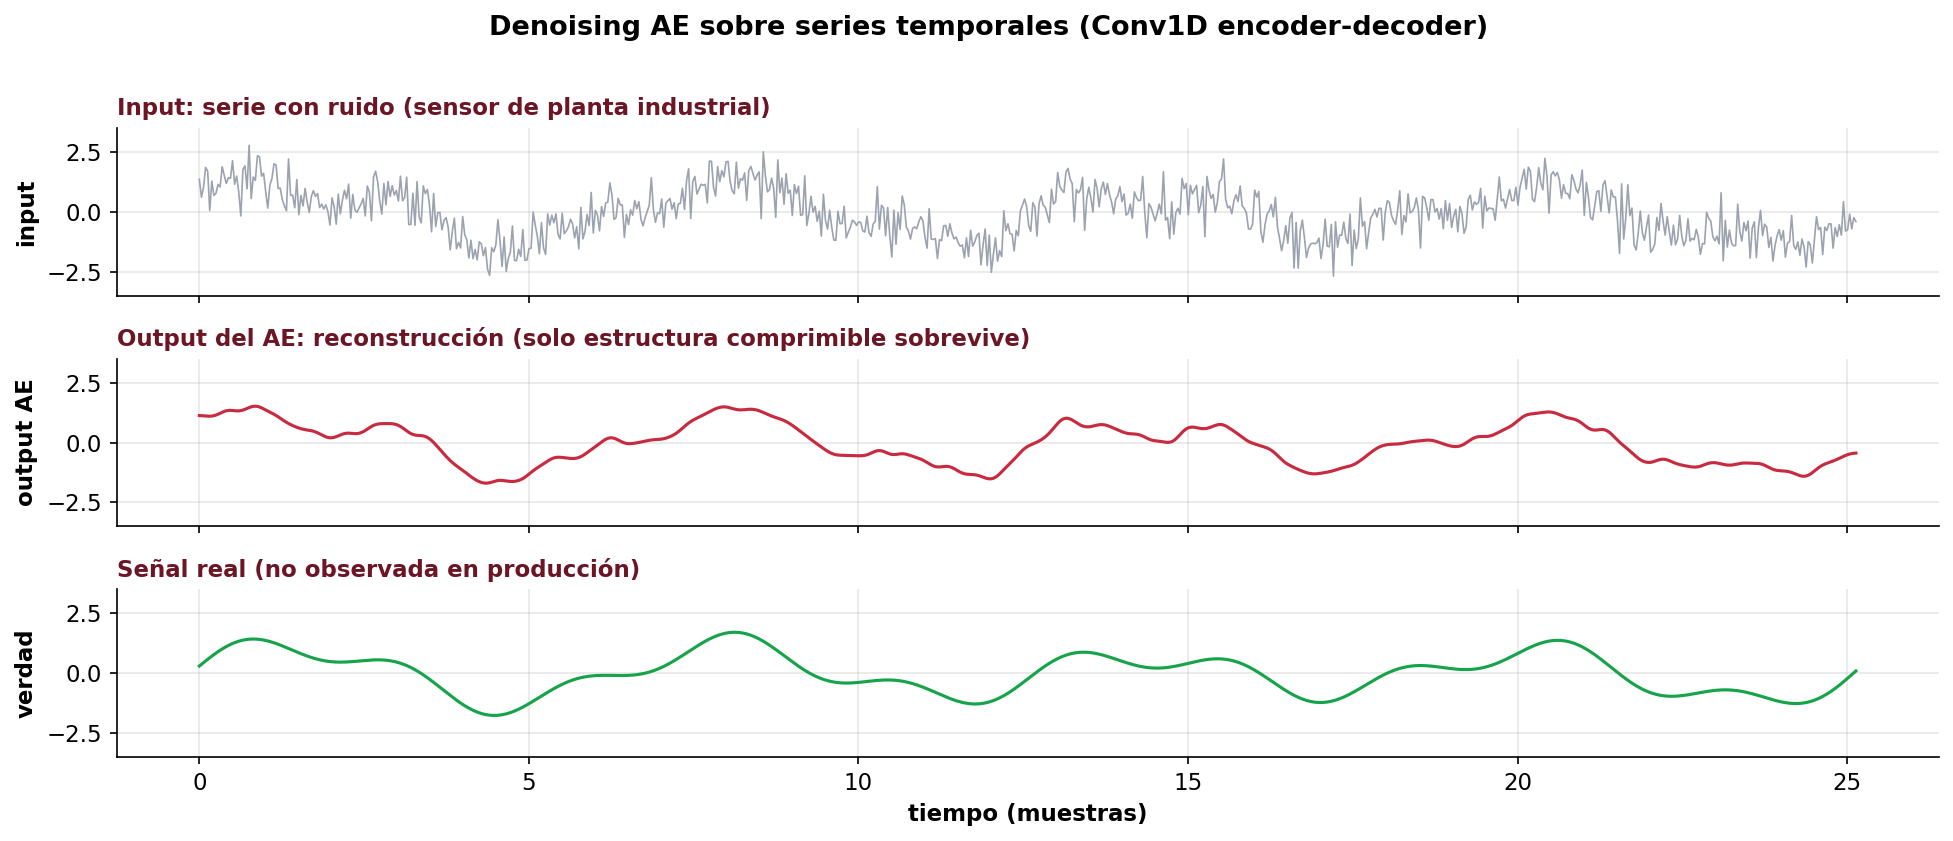
\includegraphics[width=0.95\textwidth]{fig_denoising_series.png}
  \end{center}
  \vspace{2pt}
  {\footnotesize\color{arcaDark}\bfseries
  Misma idea, otra dimensión: \texttt{Conv1D} en lugar de \texttt{Conv2D}. Para Arca: limpiar telemetría de sensores antes de un modelo de forecasting o de detección de fallas.}
\end{frame}

\begin{frame}[shrink]{Cuándo SÍ y Cuándo NO Usar Denoising AE}
  \vspace{6pt}
  {\footnotesize
  \begin{tabular}{@{}p{8.5cm} c@{}}
    \toprule
    \rowcolor{arcaLightGray}
    \textbf{Condición} & \textbf{¿Aplica?} \\
    \midrule
    Ruido y señal son estructuralmente distintos (uno comprime, el otro no) & {\color{codeGreen}\bfseries SÍ} \\
    Puedes simular el patrón de degradación con razonable fidelidad & {\color{codeGreen}\bfseries SÍ} \\
    El task downstream se beneficia de input limpio (OCR, clasificación, forecast) & {\color{codeGreen}\bfseries SÍ} \\
    \midrule
    El ``ruido'' es \emph{variabilidad legítima} del proceso que importa para el negocio & {\color{arcaRed}\bfseries NO} \\
    Métodos clásicos ya resuelven (mediana, gaussiano, EMA, Savitzky-Golay) & {\color{arcaRed}\bfseries NO} \\
    Tipo de degradación cambia con el tiempo y no puedes re-entrenar & {\color{arcaRed}\bfseries NO} \\
    Solo tienes ejemplos sucios, no pares (sucio, limpio) & {\color{arcaRed}\bfseries NO} \\
    \bottomrule
  \end{tabular}}
  \vspace{12pt}
  {\footnotesize\color{arcaDark}\bfseries
  Regla pragmática: intenta primero con un filtro clásico. Si no alcanza, sube a denoising AE.}
\end{frame}

% ═════════════════════════════════════════════════════════════════════════════
% PARTE 7: ANOMALY DETECTION
% ═════════════════════════════════════════════════════════════════════════════
\sectionframe{Parte 7}{Aplicación 3 --- Detección de Anomalías a Profundidad (ECG5000)}

\begin{frame}[shrink]{La Idea Formulada con Precisión}
  \vspace{4pt}
  \begin{center}
    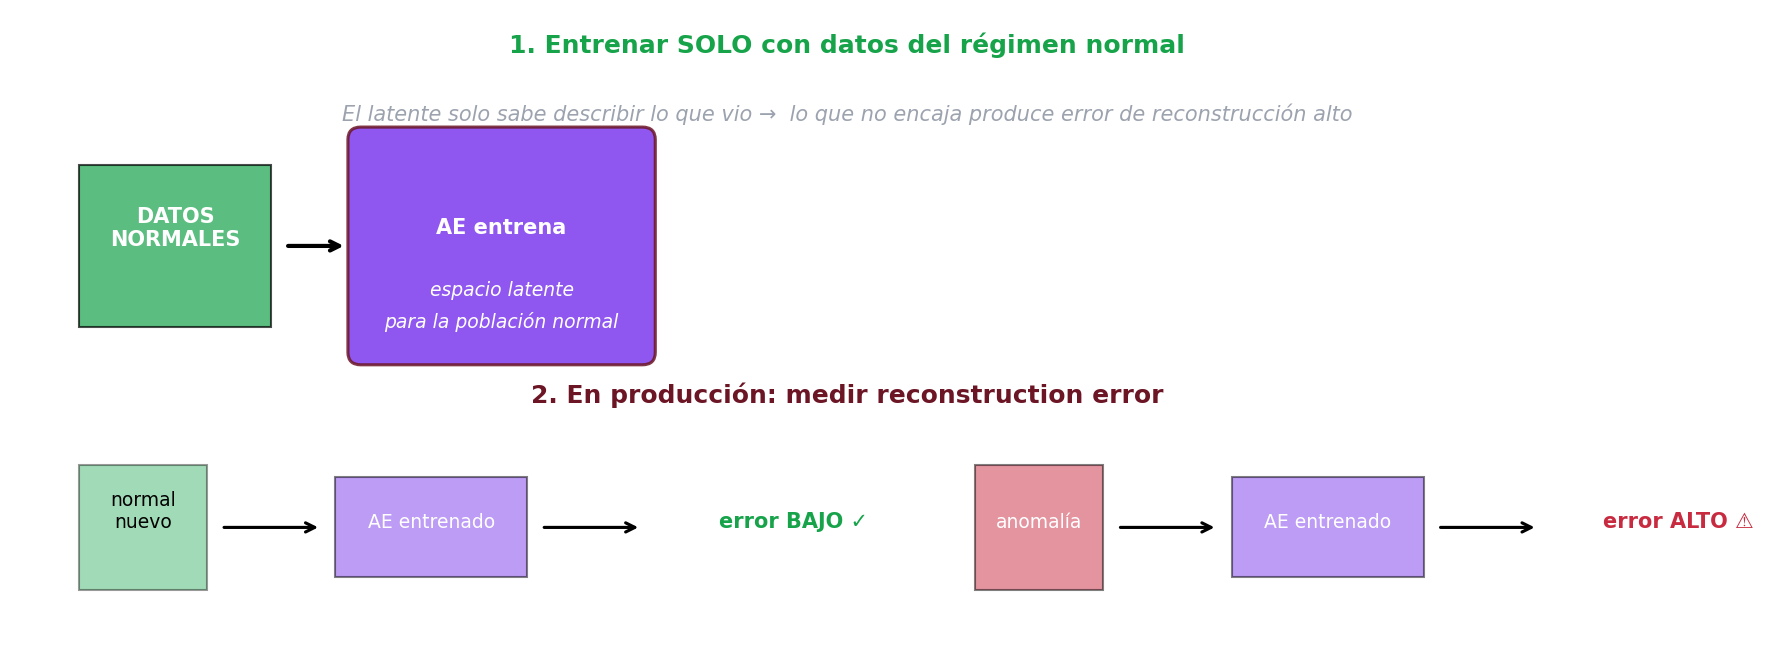
\includegraphics[width=0.94\textwidth]{fig_anomaly_concept.png}
  \end{center}
  \vspace{4pt}
  {\footnotesize\color{arcaDark}\bfseries
  Entrenamos el AE únicamente con datos del régimen normal. El espacio latente queda diseñado para describir esa población. Cuando llega algo nuevo: si encaja, baja reconstruction error; si no encaja, las coordenadas latentes no fueron parametrizadas para esa forma $\to$ error alto.}
\end{frame}

\begin{frame}[shrink]{Qué Es Exactamente el ``Error de Reconstrucción''}
  \vspace{8pt}
  \begin{center}
  $\text{error}(x) \;=\; \text{distancia}\bigl(x,\; \text{decoder}(\text{encoder}(x))\bigr)$
  \end{center}
  \vspace{8pt}
  {\footnotesize
  \begin{tabular}{@{}p{2.8cm} p{4.5cm} p{5.5cm}@{}}
    \toprule
    \rowcolor{arcaLightGray}
    \textbf{Métrica} & \textbf{Fórmula} & \textbf{Cuándo usarla} \\
    \midrule
    \textbf{MAE} & $\frac{1}{n}\sum_i |x_i - \hat{x}_i|$ & Default robusto. Lo usa el tutorial oficial de TF. Penaliza errores grandes y pequeños proporcionalmente. \\
    \textbf{MSE} & $\frac{1}{n}\sum_i (x_i - \hat{x}_i)^2$ & Penaliza fuerte los errores grandes (cuadrático). Más sensible a outliers. \\
    \textbf{SSIM} & métrica perceptual & Solo para imágenes cuando MSE/MAE no capturan defectos localizados. \\
    \bottomrule
  \end{tabular}}
  \vspace{10pt}
  {\footnotesize\color{arcaDark}\bfseries
  Ese mismo número --- un escalar por observación --- es el \emph{score de anomalía}. Toda la sección que sigue es: cómo lo calculamos, cómo lo interpretamos, cómo elegimos un umbral, cómo lo evaluamos.}
\end{frame}

\begin{frame}[shrink]{ECG5000 --- el Dataset Estándar para Enseñar Esto}
  \vspace{6pt}
  {\footnotesize
  \begin{tabular}{@{}p{4.8cm} p{8.5cm}@{}}
    \toprule
    \rowcolor{arcaLightGray}
    \textbf{Característica} & \textbf{Por qué importa} \\
    \midrule
    Real, de pacientes reales & No es sintético. Las anomalías son arritmias clínicas, no perturbaciones inventadas. \\
    Público + descarga directa & Google hostea el CSV ($\sim$5 MB). Sin Kaggle ni auth. \\
    Etiquetas binarias incluidas & Permite EVALUAR el detector (precision/recall/F1) --- lo que en producción casi nunca tenés. \\
    Tabular: 140 valores por muestra & Vale como template para CUALQUIER caso tabular: fraude, mantenimiento predictivo, telemetría. \\
    Tutorial oficial de TensorFlow & \texttt{tensorflow.org/tutorials/generative/autoencoder} usa este mismo dataset. Receta verificada que converge. \\
    \bottomrule
  \end{tabular}}
  \vspace{12pt}
  {\footnotesize\color{arcaDark}\bfseries
  Mismo patrón aplicable directamente a Arca: línea de embotellado (botella OK vs tapa torcida), mantenimiento predictivo (vibración normal vs pre-falla), fraude en TPV.}
\end{frame}

\begin{frame}[fragile,shrink]{Arquitectura y Entrenamiento}
  \vspace{-4pt}
  \begin{pyblock}
import pandas as pd
URL = "http://storage.googleapis.com/download.tensorflow.org/data/ecg.csv"
df = pd.read_csv(URL, header=None)
labels, signals = df.values[:, -1].astype(int), df.values[:, :-1].astype("float32")
signals = (signals - signals.min()) / (signals.max() - signals.min())

# Solo normales para entrenar (label == 1)
X_normal = signals[labels == 1]
X_anom   = signals[labels == 0]
X_tr_normal = X_normal[:int(0.85*len(X_normal))]   # train: solo normales
X_te_normal = X_normal[int(0.85*len(X_normal)):]   # test
X_te_anom   = X_anom                                # test anomalos

# AE Dense -- arquitectura del tutorial oficial de TensorFlow
inp = keras.Input(shape=(140,))
x = layers.Dense(32, activation="relu")(inp)
x = layers.Dense(16, activation="relu")(x)
z = layers.Dense(8,  activation="relu")(x)         # bottleneck
y = layers.Dense(16, activation="relu")(z)
y = layers.Dense(32, activation="relu")(y)
out = layers.Dense(140, activation="sigmoid")(y)
anom_ae = keras.Model(inp, out)
anom_ae.compile(optimizer="adam", loss="mae")
anom_ae.fit(X_tr_normal, X_tr_normal, epochs=30, batch_size=64)
  \end{pyblock}
\end{frame}

\begin{frame}[fragile,shrink]{Calcular el Score (Error de Reconstrucción)}
  \vspace{-4pt}
  \begin{pyblock}
# Pasar normales y anomalos por el AE entrenado
recons_n = anom_ae.predict(X_te_normal)
recons_a = anom_ae.predict(X_te_anom)

# Error de reconstruccion = MAE por observacion (UN numero por latido)
err_normal = np.mean(np.abs(X_te_normal - recons_n), axis=1)
err_anom   = np.mean(np.abs(X_te_anom   - recons_a), axis=1)

print(f"Error promedio NORMALES:  {err_normal.mean():.4f}")
print(f"Error promedio ANOMALOS:  {err_anom.mean():.4f}")
print(f"Ratio anomalia/normal:    {err_anom.mean()/err_normal.mean():.1f}x")
  \end{pyblock}
  \vspace{4pt}
  {\footnotesize\color{arcaDark}\bfseries
  Cada valor de \texttt{err\_normal[i]} o \texttt{err\_anom[i]} es el \emph{score de anomalía} de esa observación. Toda la decisión binaria viene de comparar ese score contra un umbral.}
\end{frame}

\begin{frame}[shrink]{Lo Más Importante --- el Histograma de Errores}
  \vspace{4pt}
  \begin{center}
    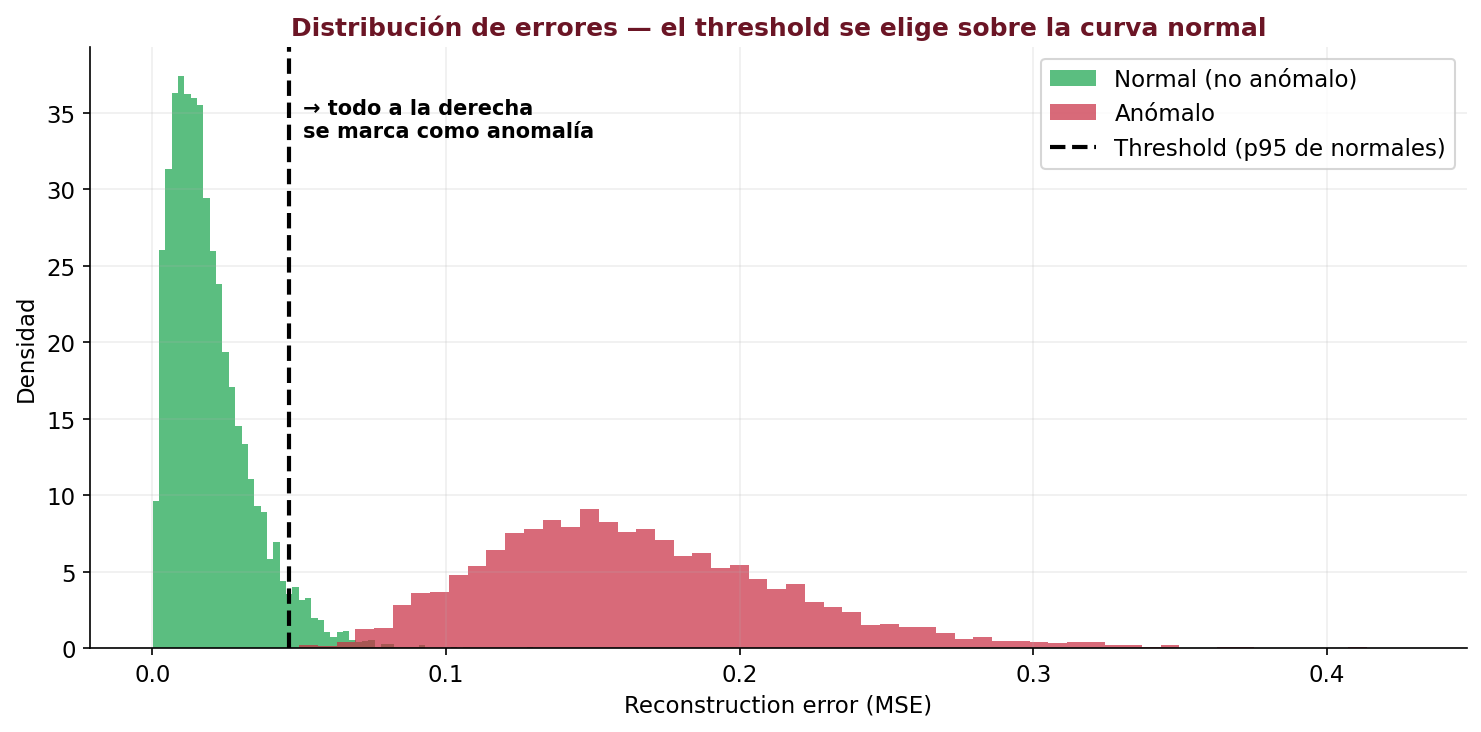
\includegraphics[width=0.75\textwidth]{fig_anomaly_hist.png}
  \end{center}
  \vspace{2pt}
  \begin{itemize}\setlength\itemsep{2pt}
    \item Si las dos distribuciones están \textbf{bien separadas}, casi cualquier umbral razonable funciona.
    \item Si se \textbf{solapan} mucho, hay trade-off precision/recall serio. Hay que decidir qué error cuesta más.
    \item La \textbf{forma de las colas} importa: anomalía sutil cae en el solape, anomalía severa está bien a la derecha.
  \end{itemize}
\end{frame}

\begin{frame}[shrink]{Elegir el Threshold --- Tres Estrategias}
  \vspace{6pt}
  {\footnotesize
  \begin{tabular}{@{}p{3.8cm} p{4.2cm} p{5.5cm}@{}}
    \toprule
    \rowcolor{arcaLightGray}
    \textbf{Estrategia} & \textbf{Cálculo} & \textbf{Cuándo usarla} \\
    \midrule
    Percentil de normales & \texttt{np.percentile(err\_n, 95)} & Default. Acepta 5\% de falsos positivos en normales conocidos. \\
    Media + k$\cdot$desviación & \texttt{err\_n.mean() + k*err\_n.std()} & Receta del tutorial oficial de TF (k=1). Asume distribución aproximadamente normal de errores. \\
    Optimizar F1 con validación & Búsqueda de umbrales que maximiza F1 con un set de validación etiquetado & Cuando tenés algunas anomalías etiquetadas y querés balancear óptimamente. \\
    \bottomrule
  \end{tabular}}
  \vspace{12pt}
  {\footnotesize\color{arcaDark}\bfseries
  El threshold es una \textbf{palanca de negocio}, no un hiperparámetro escondido. Subis $\to$ menos falsos positivos, más anomalías escapan. Bajas $\to$ más alarmas, menos anomalías perdidas.}
\end{frame}

\begin{frame}[shrink]{Métricas a Mirar para Anomaly Detection}
  \vspace{6pt}
  {\footnotesize
  \begin{tabular}{@{}p{3.0cm} p{4.0cm} p{6.5cm}@{}}
    \toprule
    \rowcolor{arcaLightGray}
    \textbf{Métrica} & \textbf{Qué mide} & \textbf{Cómo se lee en producción} \\
    \midrule
    \textbf{Precision} & TP / (TP + FP) & De cada 100 alarmas, cuántas son anomalías reales. Bajo = falsas alarmas $\to$ cansancio del operador. \\
    \textbf{Recall} & TP / (TP + FN) & De cada 100 anomalías reales, cuántas detecta. Bajo = anomalías escapan $\to$ riesgo de falla. \\
    \textbf{F1} & $2 \cdot \frac{P \cdot R}{P + R}$ & Balance entre las dos. Un número resumen. \\
    \textbf{Confusion matrix} & TP, FP, FN, TN & Detalle de los 4 cuadrantes. Lo que se reporta al cliente. \\
    \textbf{ROC AUC} & Área bajo TPR vs FPR & Capacidad discriminativa independiente del threshold. \\
    \textbf{PR AUC} & Área bajo PR & Más informativa con clases desbalanceadas (lo típico en anomalías). \\
    \bottomrule
  \end{tabular}}
  \vspace{8pt}
  {\footnotesize\color{arcaDark}\bfseries
  En ECG: Recall alto pesa más (no perder un paciente arrítmico). En fraude bancario: Precision pesa más (no bloquear clientes legítimos). Decisión de negocio, no técnica.}
\end{frame}

\begin{frame}[shrink]{Lectura de las Métricas con Threshold = p95}
  \vspace{4pt}
  {\footnotesize
  Con \texttt{threshold = np.percentile(err\_normal, 95)} sobre ECG5000, el detector típico devuelve algo así:
  }
  \vspace{8pt}
  \begin{center}
  {\footnotesize\ttfamily
  \begin{tabular}{l|cc}
                    & Pred. Normal & Pred. Anómalo \\ \hline
    Real Normal     & 388          & 21 \\
    Real Anómalo    & 60           & 2010 \\
  \end{tabular}}
  \end{center}
  \vspace{10pt}
  \begin{itemize}\setlength\itemsep{3pt}
    \item Precision (anómalo) $\approx 99\%$ --- las alarmas que dispara casi todas son arritmias reales.
    \item Recall (anómalo) $\approx 97\%$ --- de cada 100 arritmias, detecta 97.
    \item F1 $\approx 0.98$ --- detector de alta calidad sobre este dataset.
    \item ROC AUC $\approx 0.97$ --- discrimina bien para casi cualquier threshold razonable.
  \end{itemize}
\end{frame}

\begin{frame}[fragile,shrink]{Pipeline Completo en Producción}
  \vspace{-4pt}
  \begin{pyblock}
# Una funcion. Eso es todo lo que pasa cuando llega una observacion nueva.
def es_anomalia(x, modelo, threshold):
    if x.ndim == 1:
        x = x[None, :]
    x_rec = modelo.predict(x, verbose=0)
    error = float(np.mean(np.abs(x - x_rec), axis=1).item())
    return (error > threshold), error

# Uso
es_anom, score = es_anomalia(latido_nuevo, anom_ae, threshold)
if es_anom:
    alerta(f"Posible arritmia: score={score:.3f}")
  \end{pyblock}
  \vspace{4pt}
  {\footnotesize\color{arcaDark}\bfseries
  Tres líneas para inferencia. El modelo entrenado pesa pocos MB. Una T4 o incluso CPU clasifica miles de latidos por segundo.}
\end{frame}

\begin{frame}[shrink]{Consideraciones Críticas en Producción}
  \vspace{4pt}
  {\footnotesize
  \begin{tabular}{@{}p{4.7cm} p{8.5cm}@{}}
    \toprule
    \rowcolor{arcaLightGray}
    \textbf{Punto} & \textbf{Recomendación} \\
    \midrule
    Set ``normal'' realmente normal & Si se cuelan anomalías sin etiquetar, el AE las aprende como variantes normales. Limpiar con reglas o IsolationForest. \\
    Múltiples regímenes normales & Si la operación tiene varios modos (máquina arrancando vs régimen), entrenar con muestras de TODOS. \\
    Escalas distintas entre features & \texttt{StandardScaler} o \texttt{MinMaxScaler} antes. \\
    Variables categóricas & One-hot encoding primero. \\
    Bottleneck demasiado grande & Aprende la identidad. Mantener entre 1/5 y 1/20 del input. \\
    Drift del régimen normal & Re-entrenar periódicamente. Definir el ciclo desde el inicio del proyecto. \\
    Calibrar el threshold con datos de producción & El p95 sobre train es conservador. Recalibrar mejora el detector. \\
    \bottomrule
  \end{tabular}}
\end{frame}

\begin{frame}[shrink]{Cuándo NO Usar AE Para Anomalías}
  \vspace{10pt}
  \begin{itemize}\setlength\itemsep{8pt}
    \item Si tenés \textbf{muchas anomalías etiquetadas}: clasificación supervisada gana siempre.
    \item Si las anomalías son del \textbf{mismo régimen} que lo normal con variaciones sutiles: probar primero \texttt{IsolationForest} o \texttt{OneClassSVM} --- suelen ir mejor en tabular y son más interpretables.
    \item Si necesitás \textbf{explicar qué hace anómala} a una muestra: AE da el score pero no el por qué. Métodos basados en árboles dan importancia de features.
  \end{itemize}
\end{frame}

% ═════════════════════════════════════════════════════════════════════════════
% PARTE 8: U-NET
% ═════════════════════════════════════════════════════════════════════════════
\sectionframe{Parte 8}{U-Net --- el AE Que Hace Segmentación}

\begin{frame}[shrink]{Conexión con Clase 28}
  \vspace{8pt}
  \begin{itemize}\setlength\itemsep{6pt}
    \item Esta mañana entrenamos \texttt{yolo26n-seg} para contar píldoras.
    \item El \textbf{head de segmentación de YOLO es una variante de U-Net}.
    \item Y \textbf{U-Net es estructuralmente un autoencoder convolucional con \emph{conexiones laterales}} (skip connections).
    \item La arquitectura encoder-decoder que llevamos toda la clase montando es la misma idea base. Lo que cambia es el target y un detalle arquitectural.
  \end{itemize}
\end{frame}

\begin{frame}[shrink]{Arquitectura U-Net}
  \vspace{4pt}
  \begin{center}
    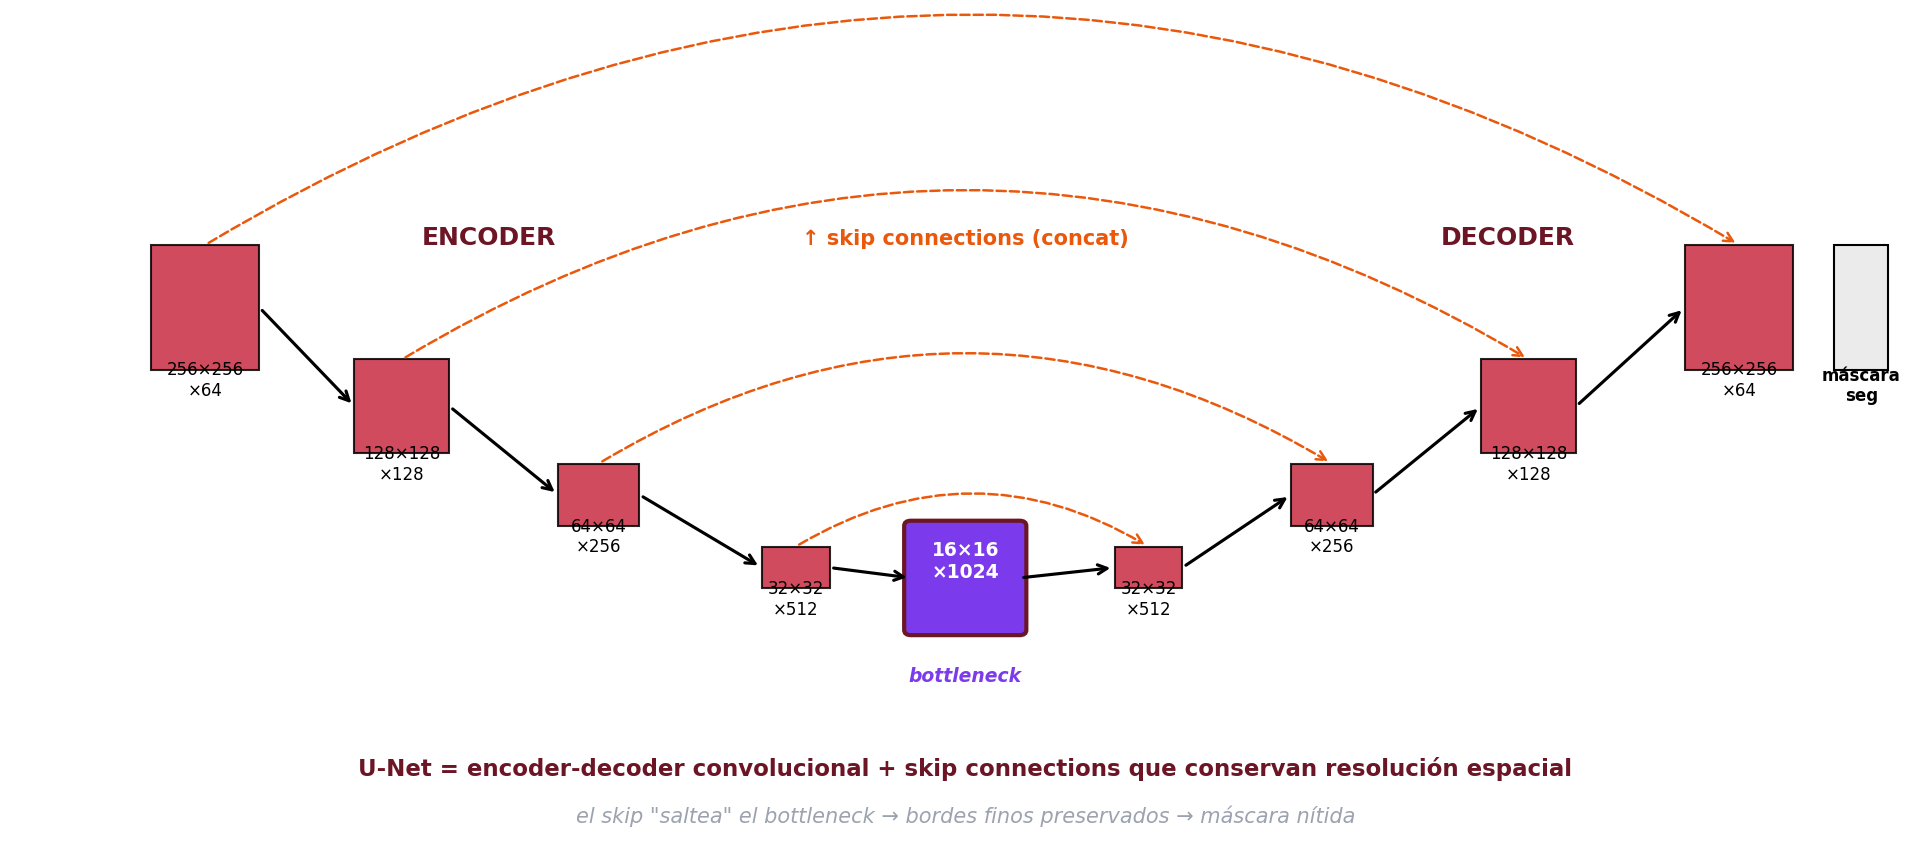
\includegraphics[width=0.96\textwidth]{fig_unet.png}
  \end{center}
  \vspace{2pt}
  \begin{itemize}\setlength\itemsep{2pt}
    \item Output = máscara pixel-wise (no reconstrucción de la imagen).
    \item Skip connections: el decoder recibe \textbf{también} los feature maps del encoder del mismo nivel.
    \item Resuelven el problema de que el bottleneck pierde resolución espacial $\to$ bordes finos preservados.
  \end{itemize}
\end{frame}

\begin{frame}[shrink]{La Familia AE → Generación Moderna}
  \vspace{4pt}
  \begin{center}
    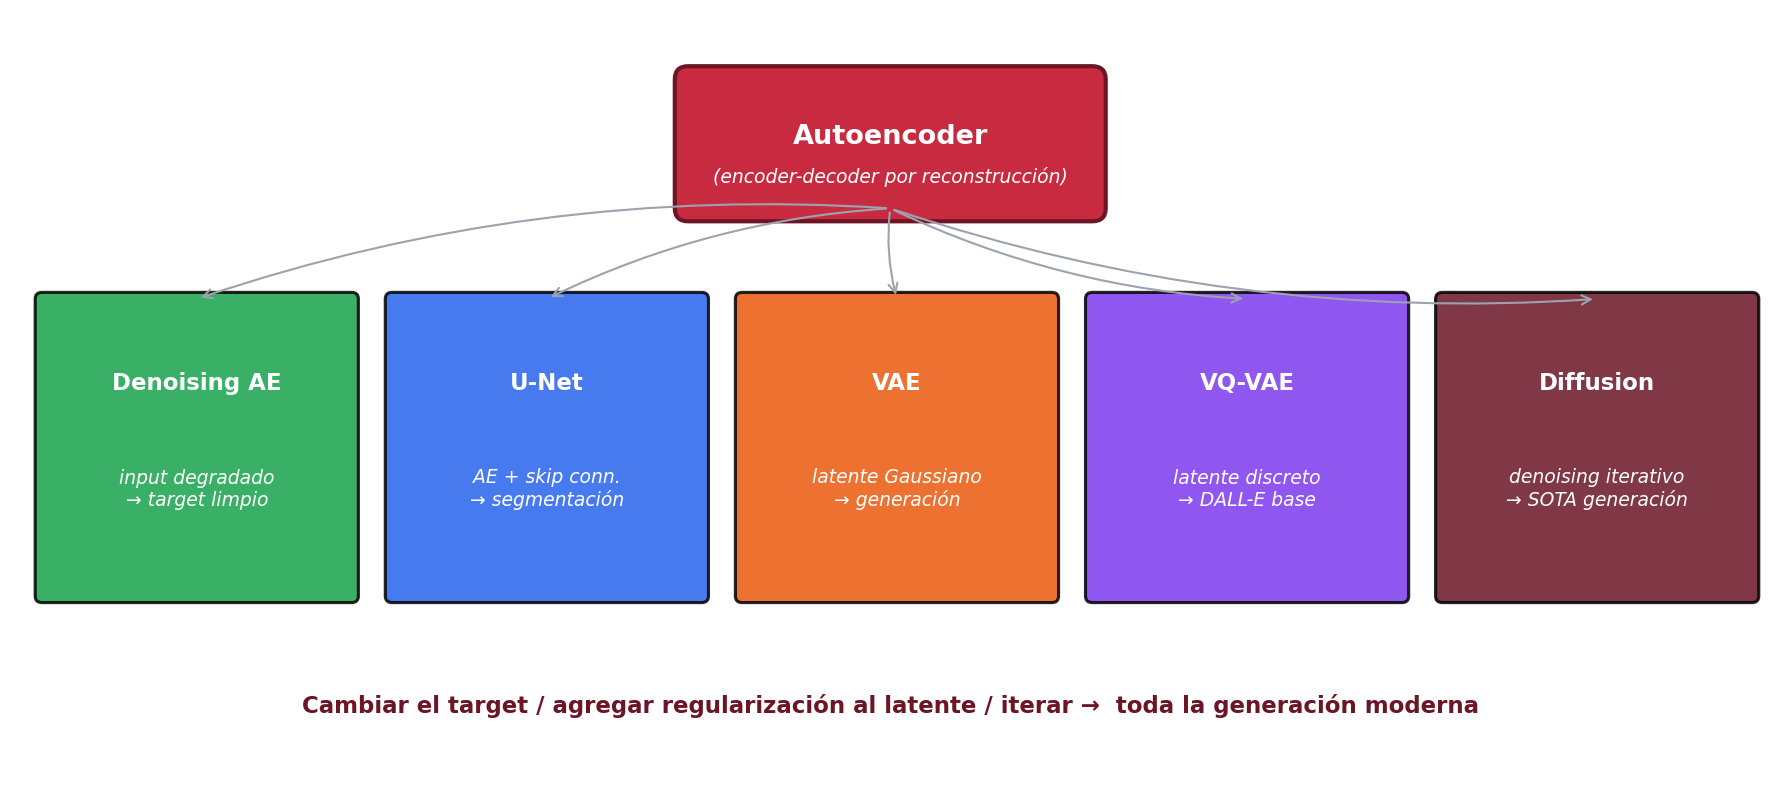
\includegraphics[width=0.96\textwidth]{fig_familia_ae.png}
  \end{center}
  \vspace{2pt}
  {\footnotesize\color{arcaDark}\bfseries
  Cambiar el target / regularizar el latente / iterar el denoising $\to$ toda la generación moderna sale de variaciones del autoencoder.}
\end{frame}

% ═════════════════════════════════════════════════════════════════════════════
% PARTE 9: CIERRE
% ═════════════════════════════════════════════════════════════════════════════
\sectionframe{Parte 9}{Cuándo Usar (y Cuándo No) un Autoencoder}

\begin{frame}[shrink]{Decisión Rápida}
  \vspace{4pt}
  \begin{center}
    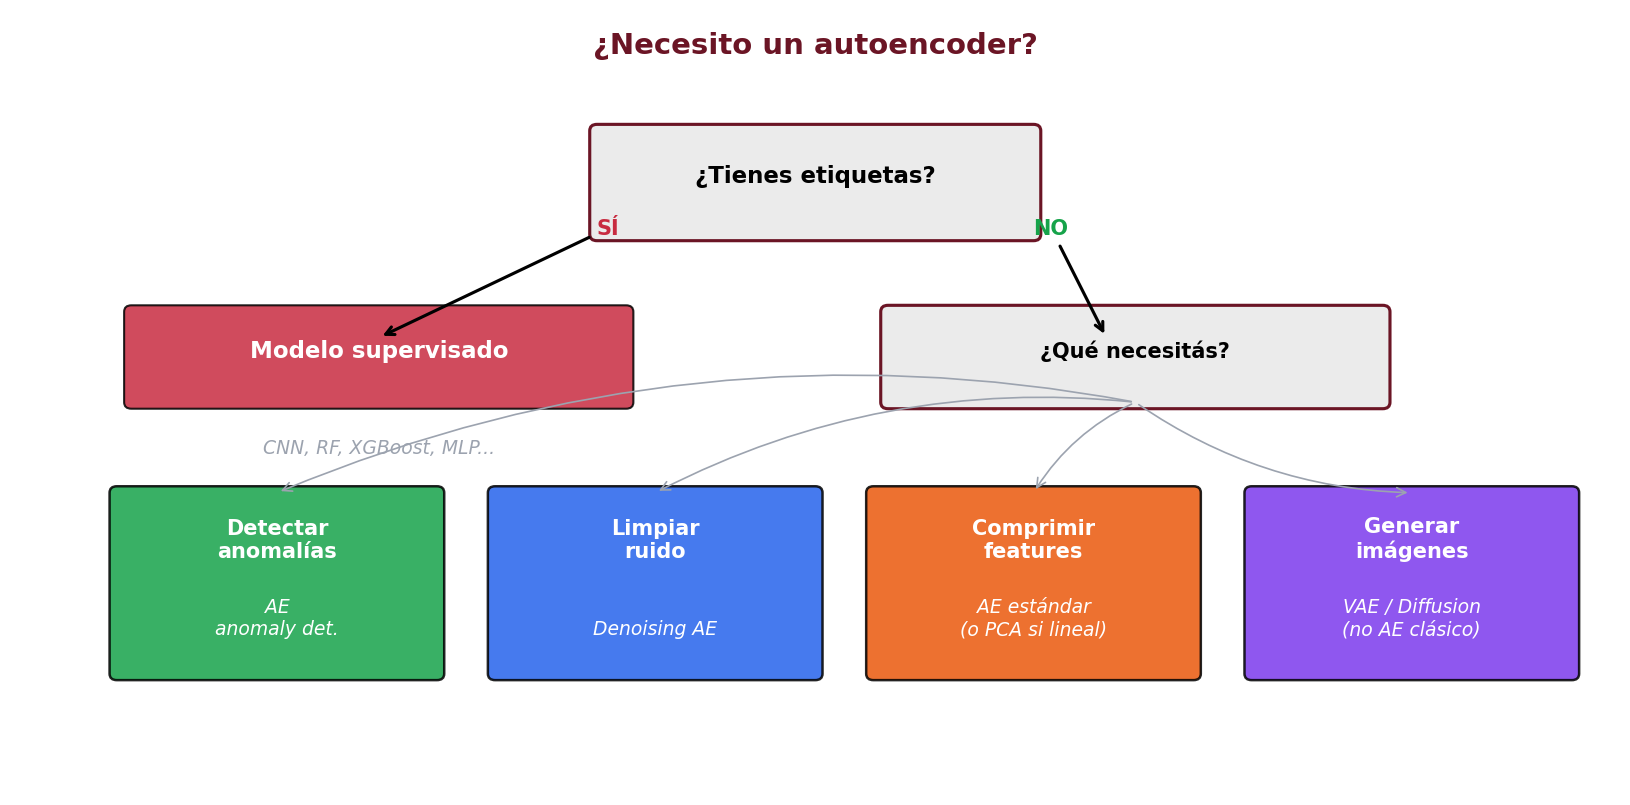
\includegraphics[width=0.96\textwidth]{fig_cuando_usar.png}
  \end{center}
\end{frame}

\begin{frame}[shrink]{Las 4 Trampas Más Comunes}
  \vspace{6pt}
  {\footnotesize
  \begin{tabular}{@{}p{4.5cm} p{9.0cm}@{}}
    \toprule
    \rowcolor{arcaLightGray}
    \textbf{Trampa} & \textbf{Cómo evitarla} \\
    \midrule
    Bottleneck demasiado grande $\to$ aprende la identidad & Mantener entre 1/4 y 1/50 del input. Si reconstruye perfecto desde el primer epoch, es señal de underfitting de la compresión. \\
    Entrenar con anomalías sin etiquetar mezcladas & Limpiar el set ``normal'' con reglas de negocio o un primer filtro de IsolationForest. \\
    MSE no captura rareza visual & Para defectos puntuales: usar SSIM, atención por región, o errores locales por máscara. \\
    Sobreajuste con poca data & Dropout en encoder, regularización L2 sobre el latente, augmentación. \\
    \bottomrule
  \end{tabular}}
\end{frame}

\begin{frame}[shrink]{Lo Que Asume Todo Autoencoder}
  \vspace{8pt}
  {\footnotesize
  \begin{tabular}{@{}p{5.0cm} p{8.5cm}@{}}
    \toprule
    \rowcolor{arcaLightGray}
    \textbf{Asunción} & \textbf{Qué pasa si falla} \\
    \midrule
    Los datos tienen regularidades comprimibles & Si son ruido puro, el AE no aprende nada útil. El histograma de errores se ve plano. \\
    Lo que quieres detectar (anomalía / ruido) NO es la mayoría & Si la ``anomalía'' es el 50\% de los datos, el AE la incorpora como variante normal. \\
    Tu loss refleja lo que importa en tu dominio & Si MSE no captura tu tipo de defecto, cambiar de loss o agregar pesos por región. \\
    \bottomrule
  \end{tabular}}
  \vspace{14pt}
  {\footnotesize\color{arcaDark}\bfseries
  Estas 3 asunciones se verifican \emph{antes} de poner el AE en producción, no después. El histograma de errores y un set de validación pequeño con anomalías conocidas son el test mínimo.}
\end{frame}

\begin{frame}[shrink]{Resumen}
  \vspace{6pt}
  \begin{itemize}\setlength\itemsep{3pt}
    \item Autoencoder = \textbf{codificación automática en un espacio latente}. Red que aprende un sistema de coordenadas propio para los datos.
    \item Régimen \textbf{auto-supervisado} ($X \to X$). Sin etiquetas.
    \item PCA = caso particular del AE lineal. Los AE generalizan a no linealidad.
    \item El \textbf{encoder entrenado} es el activo, no la reconstrucción.
    \item Aplicaciones: \textbf{denoising}, \textbf{detección de anomalías} (el caso de negocio más fuerte para Arca), \textbf{compresión de features}, \textbf{visualización}, \textbf{pretraining}.
    \item \textbf{U-Net} = AE convolucional con skip connections $\to$ segmentación.
    \item \textbf{No usar para}: clasificación con labels (supervisado gana), generación de alta calidad (VAE / Diffusion).
  \end{itemize}
\end{frame}

\begin{frame}[shrink]{Tarea Para Casa}
  \vspace{6pt}
  \begin{enumerate}\setlength\itemsep{6pt}
    \item Tomar el \textbf{Conv AE de denoising} y entrenarlo con \texttt{Fashion-MNIST}. Probar con \texttt{NOISE = 0.5} y \texttt{NOISE = 0.7}. ¿A qué nivel de ruido se rompe?
    \item Tomar el \textbf{AE de anomaly detection} y cambiar la clase ``normal'' de \texttt{0} a \texttt{1}. ¿Cambia el umbral? ¿Cuáles dígitos son los más anómalos relativos a 1?
    \item \textbf{Para los curiosos}: armar un AE tabular sobre un dataset real (sugerencia: Credit Card Fraud de Kaggle o cualquier dataset de telemetría que tengan a mano). Reportar precision / recall en detección con un threshold de p95.
  \end{enumerate}
  \vspace{10pt}
  {\footnotesize\color{arcaDark}\bfseries
  Próxima clase (miércoles 20 de mayo, clase 30): cierre del Módulo 4 --- repaso integrador del bloque de Machine Learning y transición al Módulo 5 (Modelos Avanzados): RNN, LSTM, series temporales.}
\end{frame}

% ── CIERRE ───────────────────────────────────────────────────────────────────
{
\setbeamertemplate{headline}{}
\setbeamertemplate{footline}{}
\begin{frame}[plain, noframenumbering]
  \begin{tikzpicture}[remember picture, overlay]
    \fill[arcaRed] (current page.south west) rectangle (current page.north east);
    \node[anchor=center, text=white, font=\Huge\bfseries] at
      ([yshift=0.5cm]current page.center) {Preguntas};
    \node[anchor=center, text=white!80, font=\large] at
      ([yshift=-0.8cm]current page.center)
      {Clase 29 \textbar{} Autoencoders};
  \end{tikzpicture}
\end{frame}
}

\end{document}
